\documentclass[12pt]{article}
\usepackage[a4paper,top=2cm,bottom=2cm,left=1.5cm,right=1.5cm]{geometry}
\usepackage[utf8]{vietnam}
\usepackage{graphicx}
\usepackage{wrapfig}
\usepackage{amsfonts,amsmath,amssymb}
\usepackage{siunitx}
\usepackage[hidelinks]{hyperref}
\usepackage{indentfirst}

%%%%%%%%%% EQUATION COUNTER & REFERENCE %%%%%%%%%% 
\usepackage{xassoccnt}
\newcounter{totalequations}
\DeclareAssociatedCounters{equation}{totalequations}
\let\theOldHequation\theHequation
\renewcommand{\theHequation}{\theOldHequation::\number\value{totalequations}}

%%%%%%%%%% PAGESTYLE %%%%%%%%%%
\usepackage{fancyhdr}
\pagestyle{fancy}
\fancyhf{}
\fancyhead[L]{\href{https://www.facebook.com/physicspen1111/}{\textbf{Physics Pen}}}
\fancyhead[R]{\textbf{CPhO 40 - Vòng Bán Kết}}
\fancyfoot[C]{\thepage}

\begin{document}

%%%%%%%%%% FIRST PAGE STYLE %%%%%%%%%%
\thispagestyle{empty}

%%%%%%%%%% TITLE %%%%%%%%%%
\begin{center}
  \fontfamily{cmss}\fontseries{b}\LARGE\textbf{
    Đề thi và Lời giải\\
    Olympic Vật lý Trung Quốc năm 2023\\
    Vòng Bán kết}
\end{center}

\begin{center}
  \href{https://www.facebook.com/physicspen1111/}{\large{\textit{Sưu tầm và biên soạn bởi Physics Pen}}}
\end{center}

\vspace{1cm}

%%%%%%%%%% PROBLEMS %%%%%%%%%%
\noindent\textbf{Câu I:}\\
\noindent Đĩa Faraday là một máy phát điện đơn giản, có cấu tạo bao gồm một đĩa kim loại làm bằng sắt (một loại vật liệu dẫn điện) có bán kính trong là $r_1$, bán kính ngoài là $r_2$ và độ dày là $h$. \\
\begin{figure}[H]
  \centering
  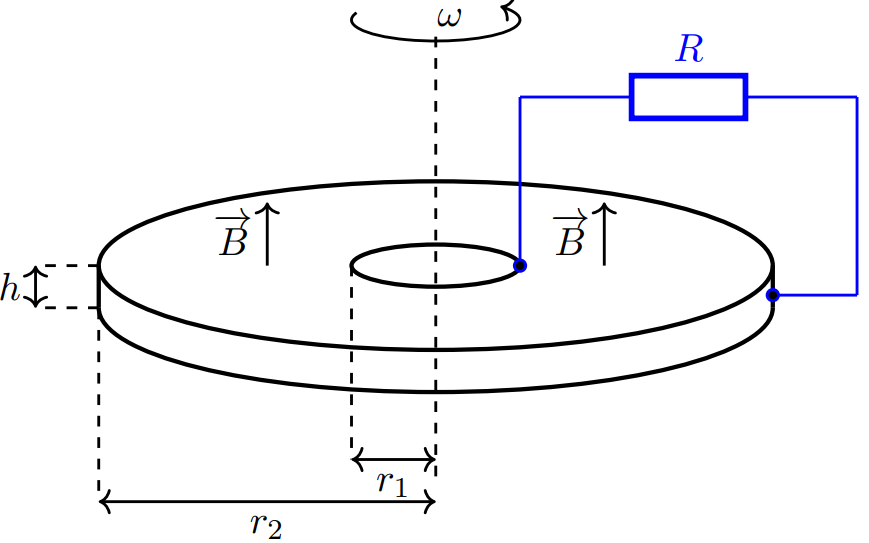
\includegraphics[width=0.5\textwidth]{Figures/Problems/Fig 1.1.png}
  \begin{center}
    \figurename{ 1}
  \end{center}
\end{figure}
\vspace{-0.5cm}
\noindent Đĩa được đặt trong một từ trường đều không đổi có cảm ứng từ $\vec{B}$ theo phương vuông góc với mặt phẳng của đĩa như được biểu diễn trong hình vẽ. Độ dẫn điện của sắt là $\sigma$.

\subsubsection*{Phần A: Mạch hở}
\noindent Trong phần này, người ta cho đĩa quay với tốc độ góc không đổi $\omega$ như Hình 1. Lúc này, đĩa chưa được nối với điện trở $R$ (không có đoạn mạch màu xanh dương).
\begin{enumerate}
  \item Xác định điện trường $\vec{E}$ bên trong đĩa và hiệu điện thế $V_0$ giữa mép trong và mép ngoài của đĩa. \textit{Gợi ý:} Trong một vật dẫn ở trạng thái cân bằng tĩnh điện, hợp lực tác dụng lên các điện tích tự do bằng không.
  \item Tìm điện trở $R_0$ của đĩa.
\end{enumerate}

\subsubsection*{Phần B: Phát điện}
\noindent Bây giờ, mép trong và mép ngoài của đĩa được nối với một điện trở $R$ như được minh họa bằng màu xanh dương trong hình vẽ. Các tiếp điểm không quay cùng với đĩa. Giả sử các tiếp điểm không có điện trở. Bỏ qua mọi ma sát.
\begin{enumerate}
  \item Xác định hiệu điện thế $V$ giữa mép trong và mép ngoài của đĩa. \textit{Gợi ý:} Lúc này, đĩa hoạt động như một nguồn điện không lý tưởng.
  \item Tính tổng công suất $P_0$ và công suất điện $P$ của nguồn.
  \item Tìm hiệu suất $\eta$ của máy phát.
  \item Tìm công suất điện cực đại $P_{\text{max}}$ và hiệu suất của nguồn khi hoạt động tại công suất đầu ra này.
\end{enumerate}

\subsubsection*{Phần C: Phanh tái sinh}
\noindent $N$ đĩa Faraday được dùng làm bánh xe và được kết nối cơ học với một đoàn tàu. Đoàn tàu có khối lượng $M = 400$ tấn và điện trở hiệu dụng $R$, mỗi bánh xe có khối lượng $m = 30$ kg. Phần duy nhất của tàu có chuyển động quay là các bánh xe. Sắt có độ dẫn điện $\sigma = 1{,}0 \cdot 10^7~\Omega^{-1} \cdot m^{-1}$, nhiệt dung riêng $c = 4{,}5 \cdot 10^2~J\,kg^{-1}\,K^{-1}$ và nhiệt độ nóng chảy $T = 1800~\text{K}$.
\begin{enumerate}
  \item Biểu diễn động năng của đoàn tàu dưới dạng $E = \frac{1}{2}I_{\text{eff}}\omega^2$ theo các đại lượng đã cho khi bánh xe quay với tốc độ góc $\omega$. Tìm $I_{\text{eff}}$. \textit{Gợi ý:} Moment quán tính của một vành tròn có khối lượng $M$, bán kính trong $R_1$ và bán kính ngoài $R_2$ đối với trục quay đi qua tâm và vuông góc với mặt phẳng vành là
        \begin{equation*}
          \frac{1}{2} M(R_2^2 + R_1^2)
        \end{equation*}
  \item Xác định động năng của đoàn tàu trong trường hợp $M \gg Nm$.
  \item Trong các ý còn lại của phần C, bạn có thể giả sử rằng $M \gg Nm$.
  \item Xác định tốc độ góc $\omega$ tại thời điểm $t$.
  \item Mất bao lâu để tốc độ của tàu giảm đi một nửa?
  \item Nếu tàu được hãm bằng cách nối tắt vành trong với vành ngoài của đĩa (lúc này $R = 0$), hãy ước lượng số lượng bánh xe tối thiểu để chúng không bị nóng chảy.
  \item Gia tốc khi hãm phanh có an toàn cho hành khách không? Lấy $B = 0{,}1\,$T, $r_1 = 10\,$cm, $r_2 = 50\,$cm và $h = 1{,}0\,$cm.
\end{enumerate}

\noindent\textbf{Câu II:}\\
\begin{wrapfigure}{r}{9cm}
  \centering
  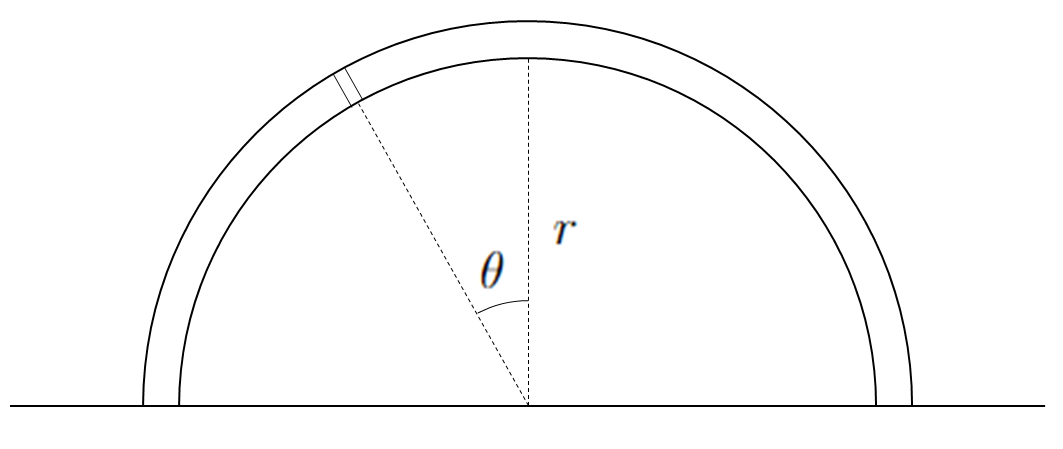
\includegraphics[width=0.5\textwidth]{images/Hinh 2.PNG}
  \vspace{-25px}
  \begin{center}
    \figurename{ 2}
  \end{center}
  \vspace{15px}
\end{wrapfigure}

\vspace{-30px}
\noindent Một ống thuỷ tinh mỏng, tiết diện đều, hai đầu bịt kín được uốn thành một nửa đường tròn bán kính $r$ (bán kính tiết diện của ống rất nhỏ so với $r$) sau đó được gắn cố định trên trên mặt sàn nằm ngang sao cho toàn bộ ống nằm trong mặt phẳng thẳng đứng như hình 2. Bên trong ống có một piston mỏng có khối lượng $m$ được làm bằng kim loại, diện tích của piston bằng với tiết diện của ống thuỷ tinh. Đường nối tâm đường tròn và vị trí của piston hợp với phương thẳng đứng một góc $\theta$. Hai bên piston đều chứa n mol khí lý tưởng, giả sử nhiệt độ của khí luôn bằng nhiệt độ $T$ của môi trường bên ngoài. Cho biết gia tốc trọng trường có độ lớn $g$, hằng số khí lý tưởng $R$, xem như tất cả các quá trình biến đổi trạng thái của khí đều chuẩn tĩnh. Bỏ qua mọi ma sát.\\
\vspace{-15pt}
\begin{enumerate}
  \item Khi nhiệt độ $T$ lớn hơn một nhiệt độ tới hạn $T_{C}$ nào đó, vị trí cân bằng bền của piston nằm ngay chính giữa ống ($\theta=0$). Hãy tìm biểu thức của $T_{C}$ và xác định tần số góc trong dao động bé của piston quanh vị trí cân bằng này.
  \item Khi $T=T_{C}$, hãy đánh giá tính ổn định của piston khi nó nằm cân bằng ở giữa ống ($\theta=0$).\\
\end{enumerate}
\vspace{-15px}
\noindent Đối với các câu hỏi bên dưới, xem $T_{C}$ như một thông số đã biết và không cần thay vào giá trị mà bạn đã tìm được ở ý 1.
\begin{enumerate}
  \setcounter{enumi}{2}
  \item Khi $T<T_{C}$, piston cân bằng tại vị trí góc $\theta_{0}$, tìm phương trình mà $\theta_{0}$ phải thoả mãn. Xác định biểu thức gần đúng khi nhiệt độ $T$ giảm nhẹ (xấp xỉ đến bậc thấp nhất khác 0).
  \item Khi $T<T_{C}$, xác định tần số góc $\omega_{0}$ trong dao động bé của piston quanh vị trí cân bằng tại $\theta_{0}$, tần số này bằng bao nhiêu khi nhiệt độ của khí lớn hơn và nhỏ hơn $T_{C}$ một chút.
  \item Khi $T<T_{C}$, giả sử vận tốc ban đầu của piston gần như bằng không, hãy tìm độ lớn vận tốc góc của piston khi nó di chuyển từ vị trí chính giữa $(\theta=0)$ đến vị trí góc lớn nhất $\theta$ mà nó có thể đi được.
\end{enumerate}

\noindent\textbf{Câu III:}\\
\vspace{-1cm}
\begin{wrapfigure}[16]{r}{7cm}
  \centering
  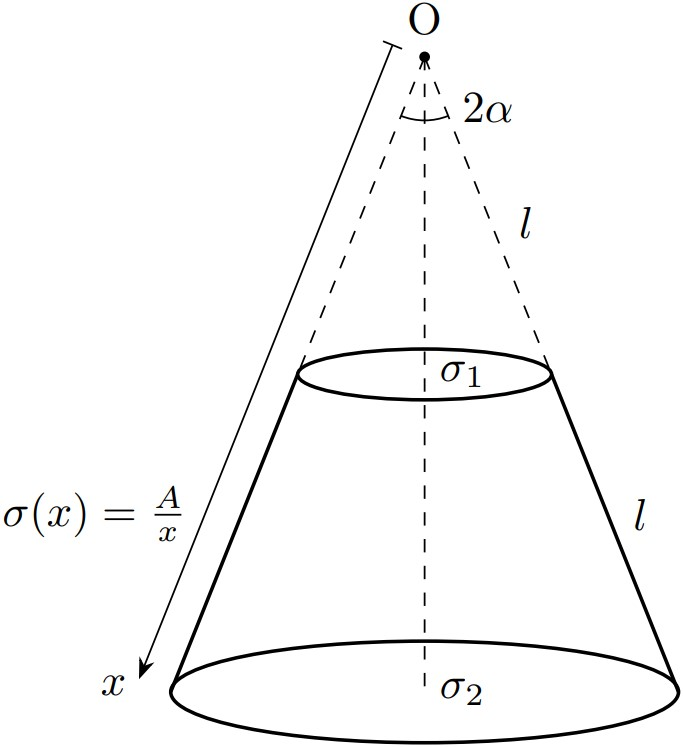
\includegraphics[width=0.38\textwidth]{Figures/Fig 3.jpg}
  \begin{center}
    \figurename{ 3}
  \end{center}
\end{wrapfigure}

\noindent Một khối đặc có dạng nón cụt, không dẫn điện, được tích điện trên mặt bên sao cho mật độ điện tích mặt thay đổi theo khoảng cách $x$ đến đỉnh $O$ theo công thức $\sigma(x)=A/x$ với $A$ là một hằng số dương đã biết. Đáy trên và đáy dưới của hình nón cụt được tích điện đều với mật độ điện tích tương ứng là $\sigma_{1}$ và $\sigma_{2}$. Độ dài đường sinh và nửa góc ở đỉnh của hình nón đầy đủ lần lượt là $2l$ và $\alpha=30^{\circ}$, độ dài đường sinh của hình nón cụt là $l$.
\begin{enumerate}
  \item Giả sử $\sigma_{1}=-\sigma_{2}=\sigma_{0}$ với $\sigma_{0}$ là một giá trị đã biết. Xác định độ lớn điện trường $E_{O}$ tại điểm $O$ trên hình 3.
\end{enumerate}
Bên trong hình nón cụt, người ta đục một lỗ nhỏ dọc theo trục đối xứng của nó. Một điện tích thử $-q$ với $q>0$, khối lượng $m$, có thể di chuyển không ma sát bên trong lỗ này. Giả sử $\sigma_{1}=\sigma_{2}=\sigma_{0}$.
\begin{enumerate}
  \setcounter{enumi}{1}
  \item Xác định khoảng cách từ vị trí cân bằng của điện tích thử bên trong hình nón cụt tới điểm $O$. Đồng thời, hãy chỉ ra rằng, khoảng cách này không phụ thuộc vào $\sigma_{0}$.
  \item Với giá trị nào của $\sigma_{0}$ thì cân bằng của điện tích thử ở vị trí vừa tìm được ở ý trên là bền? Tìm chu kỳ dao động bé của điện tích thử quanh vị trí cân bằng này.
\end{enumerate}
Trong suốt bài toán, hình nón cụt được giữ cố định. Cho biết hằng số điện môi của vật liệu làm nên hình nón cụt là $\varepsilon=1$, bỏ qua tác dụng của trọng lực và các hiện tượng từ tính.\\

\noindent\textbf{Câu IV:}\\
\vspace{-1cm}
\begin{wrapfigure}[13]{r}{5cm}
  \centering
  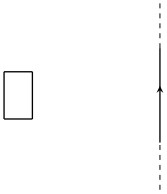
\includegraphics[width=0.25\textwidth]{Figures/Fig 4.jpg}
  \begin{center}
    \figurename{ 4}
  \end{center}
\end{wrapfigure}

\noindent Một khung dây cứng, mảnh hình chữ nhật có thể di chuyển trên bề mặt nằm ngang và nhẵn, trên bề mặt có gắn cố định một sợi dây thẳng, mảnh, và dài vô hạn như hình 4. Ban đầu, cường độ dòng điện trong dây dẫn và khung dây bằng không. Khung dây nằm yên ở vị trí sao cho một cặp cạnh của nó song song với dây dẫn và khoảng cách giữa dây dẫn và cạnh gần nhất của khung dây rất lớn so với kích thước của khung. Sau đó, cường độ dòng điện trong dây dẫn được tăng lên đến một giá trị cực đại nào đó và được giữ không đổi ở giá trị này. Giả sử thời gian thực hiện là rất ngắn, đủ để bỏ qua chuyển động của khung dây trong quá trình này. Khi cường độ dòng điện trong dây dẫn đạt giá trị cực đại, vận tốc của khung dây là $v_{0}$. Bỏ qua độ tự cảm của khung và xem như điện trở của khung không đổi. Biết rằng sau một khoảng thời gian rất dài kể từ khi cường độ dòng điện trong dây dẫn đạt giá trị cực đại, vận tốc của khung không đổi và bằng $v_{1}$. Tìm $v_{1}$.\\

\noindent\textbf{Câu V:}\\
\vspace{-1cm}
\begin{wrapfigure}[15]{r}{7cm}
  \centering
  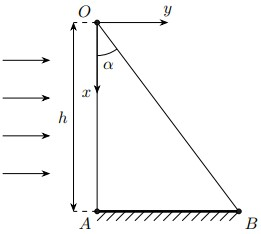
\includegraphics[width=0.38\textwidth]{Figures/Fig 5.jpg}
  \begin{center}
    \figurename{ 5}
  \end{center}
\end{wrapfigure}

\noindent Nhà thí nghiệm Gluck đã tiến hành một thí nghiệm quang học sử dụng một lăng kính đặc có tiết diện mặt cắt là tam giác vuông $OAB$ với các cạnh góc vuông là $AB$ và $OA=h$. Tất cả các mặt của lăng kính đều song song hoặc vuông góc với mặt phẳng hình vẽ. Nếu ta sử dụng hệ toạ độ $Oxy$ như được chỉ ra trên hình $5$, chiết suất của vật liệu làm lăng kính thay đổi theo công thức:
\begin{equation*}
  n(x)=\frac{3}{2-\dfrac{x}{h}}
\end{equation*}
Gluck quyết định chiếu một chùm sáng song song lên mặt bên $OA$ của lăng kính. Mặt đáy $AB$ được phủ một lớp vật liệu có khả năng hấp thụ toàn bộ ánh sáng đi qua nó. Lăng kính được đặt trong không khí, giả sử chiết suất của không khí bằng 1. Chỉ xét có tia sáng đi vào lăng kính thông qua mặt bên $OA$.
\begin{enumerate}
  \item Xét một tia sáng đi vào lăng kính tại điểm có toạ độ $x_{0}$. Xác định phương trình quỹ đạo của tia sáng đó bên trong lăng kính.
  \item Với những giá trị nào của góc $\hat{AOB}=\alpha$, các tia sáng sẽ đi qua mọi điểm trên mặt bên $OB$ của lăng kính?
  \item Với những giá trị nào của góc $\alpha$, tất cả các tia sáng khi đạt tới mặt bên $OB$ của lăng kính đều bị khúc xạ và đi ra không khí?
\end{enumerate}

\noindent\textbf{Câu VI:}\\
\begin{wrapfigure}{r}{8cm}
  \centering
  \vspace{-30px}
  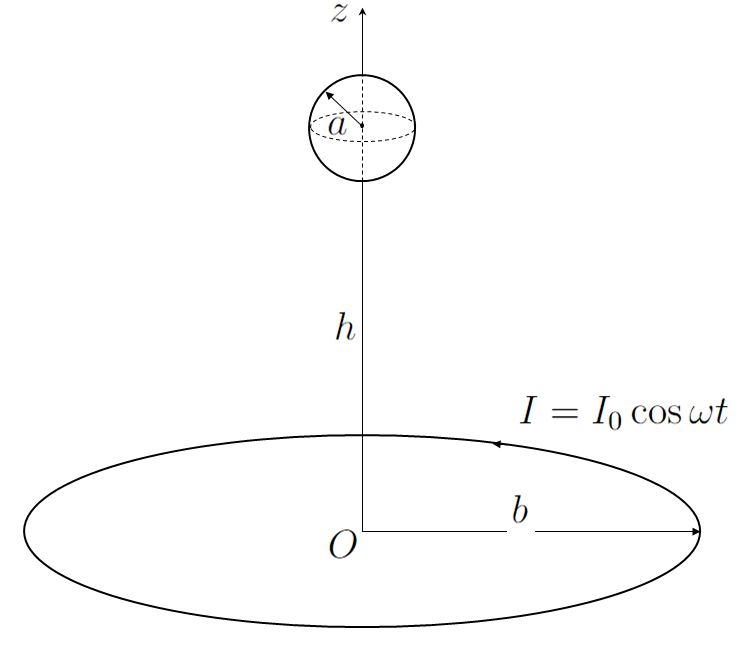
\includegraphics[width=0.45\textwidth]{images/Hinh 6.PNG}
  \vspace{-20px}
  \begin{center}
    \figurename{ 6}
  \end{center}
\end{wrapfigure}

\vspace{-30px}
\noindent Khi một vật dẫn điện được đặt trong từ trường biến thiên, dòng điện Foucault (dòng điện xoáy) sẽ xuất hiện bên trong nó. Dòng Foucault có thể tạo ra tác dụng nhiệt được sử dụng để nung nóng và rèn kim loại; bên cạnh đó, tác dụng cơ của dòng điện này còn được ứng dụng để hãm chuyển động, truyền động, treo các vật thể dẫn điện,\dots. Để nghiên cứu hai tác dụng nêu trên của dòng điện xoáy, ta sẽ sử dụng một thiết bị như hình 6: một cuộn dây bán kính $b$ được đặt cố định trên mặt bàn nằm ngang, mang dòng điện xoay chiều có cường độ $I(t)=I_{0}\cos\omega t$. Một quả cầu dẫn điện có trọng lượng $G$, bán kính $b$, độ dẫn điện $\sigma$ được đặt sao cho tâm quả cầu nằm trên trục đối xứng của vòng dây, cách tâm vòng dây một khoảng $h\ll a$. Giả sử $a\ll b$ và độ sâu bề mặt của quả cầu là $\sigma=\sqrt{\dfrac{2}{\omega\mu_{9}\sigma}}\ll a$ với $\mu_{0}$ là độ từ thẩm trong chân không. Bỏ qua hiện tượng bức xạ điện từ.
\begin{enumerate}
  \item Đặt một quả cầu dẫn lý tưởng $(\sigma)\rightarrow\infty$ bán kính $a$ trong một từ trường đều và ổn định $\vec{B}_{e}=B_{e}\hat{z}$, dòng điện từ hoá bên trong quả cầu sẽ tạo ra một từ trường $\vec{B}'$ bên ngoài quả cầu, từ trường này tương tự với từ trường do một lưỡng cực từ lý tưởng đặt tại tâm quả cầu tạo ra:
        \begin{equation*}
          \vec{B}'=\frac{\mu_{0}}{4\pi}\frac{3(\vec{m}\cdot\hat{r})\hat{r}-\vec{m}}{r^{3}}
        \end{equation*}
        trong đó $\vec{m}$ là momen lưỡng cực từ của lưỡng cực, cũng là momen lưỡng cực của quả cầu dẫn lý tưởng này. Xem $\vec{B}_{e}$ như một đại lượng đã biết, xác định $\vec{m}$ và phân bố dòng điện trên bề mặt quả cầu dẫn.
  \item Xác định cảm ứng từ $\vec{B}$ do dòng điện trong dây dẫn tạo ra tại tâm quả cầu vào thời điểm $t$.
  \item Xác định giá trị của $I_{0}$ để quả cầu có thể cân bằng tại vị trí như hình 6. Giả sử $I_{0}$ đủ lớn để biên độ dao động của quả cầu dẫn quanh vị trí cân bằng có thể bỏ quả. Cho biết: Nếu momen từ $\vec{m}$ của lưỡng cực từ và từ trường ngoài $\vec{B}_{e}$ tại vị trí của lưỡng cực có phương song song với $Oz$, các thành phần tương ứng của chúng là $m$ và $B_{e}=B_{e}(z)$ thì lực tác dụng lên lưỡng cực có dạng:
        \begin{equation*}
          \vec{F}=m\frac{dB_{e}}{dz}\hat{z}
        \end{equation*}
  \item Khi khảo sát tác dụng nhiệt của dòng điện xoáy, ta phải xét đến hiệu ứng bề mặt của quả cầu dẫn. Giả sử dòng điện xoáy được phân bố đều trên phương bán kính trong độ sâu bề mặt và bằng không ở mọi nơi khác bên trong quả cầu. Xác định biểu thức gần đúng của nhiệt năng trung bình do quả cầu toả ra trong một chu kỳ.
\end{enumerate}

\noindent\textbf{Câu VII:}\\
\noindent Tầng thấp nhất của khí quyển là tầng đối lưu, có độ dày khoảng \SI{10}{\kilo\metre}. Trong tầng đối lưu, khi càng lên cao thì nhiệt độ không khí càng giảm. Bên trên tầng đối lưu là tầng bình lưu, trong khoảng \SI{10}{\kilo\metre}, nhiệt độ gần như không thay đổi theo độ cao. Phía trên tầng bình lưu, trong một khoảng độ cao nhất định, nhiệt độ khí quyển lại tăng dần theo độ cao, tầng này được gọi là tầng nghịch (Hình 7).
\begin{enumerate}
  \item Do ánh nắng Mặt Trời, nhiệt độ không khí gần mặt đất cao hơn. Sự thay đổi nhiệt độ khí quyển trong tầng đối lưu có thể xem là kết quả của quá trình biến đổi đoạn nhiệt của không khí. Xác định mối liên hệ giữa nhiệt độ không khí và độ cao tính từ mặt đất. Giả sử nhiệt độ không khí ngay sát mặt đất là $T_{0}$, không khí là khí lý tưởng có khối lượng mol $\mu$, hệ số đoạn nhiệt $\gamma$, và hằng số khí lý tưởng $R$. Gia tốc trọng trường trong tần đối lưu có thể xem là hằng số và bằng $g$.
  \item Vận tốc truyền âm trong không khí dược tính bởi $v_{s}=\sqrt{\left(\dfrac{dp}{d\rho}\right)_{S}}$, trong đó $p$ là áp suất và $\rho$ là khối lượng riêng của không khí. Bỏ qua ảnh hưởng của gió, xác định mối liên hệ giữa vận tốc âm thanh và nhiệt độ $T$ của không khí. Nhiệt độ này thay đổi như thế nào theo độ cao?
  \item Khi sóng âm truyền trong các môi trường có vận tốc âm thanh khác nhau, nó cũng xảy ra hiện tượng phản xạ và khúc xạ, các hiện tượng này xảy ra tương tự với hiện tượng phản xạ và khúc xạ ánh sáng. Để đơn giản hoá, ta có thể coi bề mặt phân cách giữa các lớp khí quyển là phẳng, giả sử nhiệt độ trong tầng đối lưu, tầng nghịch là \SI{-10}{\celsius} và trong tầng bình lưu là \SI{-55}{\celsius}. Trong mô hình này, xét một nguồn âm trong tầng bình lưu, các sóng âm phát ra sẽ đi tới mặt phân cách giữa tầng bình lưu và tầng đối lưu (hay tầng nghịch). Hãy phân tích hiện tượng phản xạ và khúc xạ của sóng âm ứng với các góc tới khác nhau: trong trường hợp nào thì xảy ra khúc xạ?, trong trường hợp nào thì xảy ra phản xạ toàn phần? Đồng thời, vẽ sơ đồ truyền sóng âm cho từng trường hợp. Biết \SI{0}{\celsius}=\SI{273,15}{\kelvin}.
  \item Tiếp tục đơn giản hoá, giả sử nhiệt độ khí quyển không thay đổi theo độ cao, các mặt phân cách là các mặt cầu đồng tâm, nhiệt độ của tầng đối lưu và tầng nghịch giống nhau và đều cao hơn nhiệt độ của tầng bình lưu. Xét một nguồn âm và một khí cầu có gắn một đầu thu âm thanh, cả hai đều có thể ở trong tầng đối lưu hoặc tầng bình lưu. Bỏ quả sự phản xạ sóng âm trên mặt đất cũng như sự hấp thụ năng lượng của sóng âm trong khí quyển. Với 4 trường hợp khác nhau khi nguồn âm và đầu thu nằm lần lượt trong tầng đối lưu và tầng bình lưu, hãy xác định trong trường hợp nào khí cầu có thể phát hiện âm thanh từ khoảng cách xa (vài nghìn \SI{}{\kilo\metre}), và trong trường hợp nào khí cầu chỉ có thể phát hiện âm thanh từ khoảng cách ngắn (dưới \SI{1000}{\kilo\metre}). Giải thích thông qua các tính toán định lượng. Cho biết bán kính Trái Đất và khoảng $R_{e}=$\SI{6371}{\kilo\metre}.
\end{enumerate}

\noindent\textbf{Câu VIII:}\\
\noindent Bằng cách sử dụng quang phổ tia X và phổ quang điện tử, ta có thể thu được thông tin về cấu trúc của vật chất. Sơ đồ bố trí thiết bị thí nghiệm được chỉ ra trong hình 8. Ống tia X bao gồm một cathode của súng điện tử và một anode kim loại. Các electron phát ra từ cathode sẽ được tăng tốc bởi điện áp, sau đó va chạm với anode kim loại để tạo ra tia X (không tính đến bức xạ trước khi electron va chạm với anode). Phổ của nó bao gồm phổ liên tục của bức xạ hãm và phổ đặc trưng rời rạc. Trong thí nghiệm, người ta sử dụng tia X có bước sóng nhất định để tương tác với bia vật liệu, sau đó sử dụng đầu thu quang phổ tia X và đầu thu phổ quang điện tử để phát hiện tia X và quang điện tử phát ra.
\newpage

\begin{figure}[h]
  \centering
  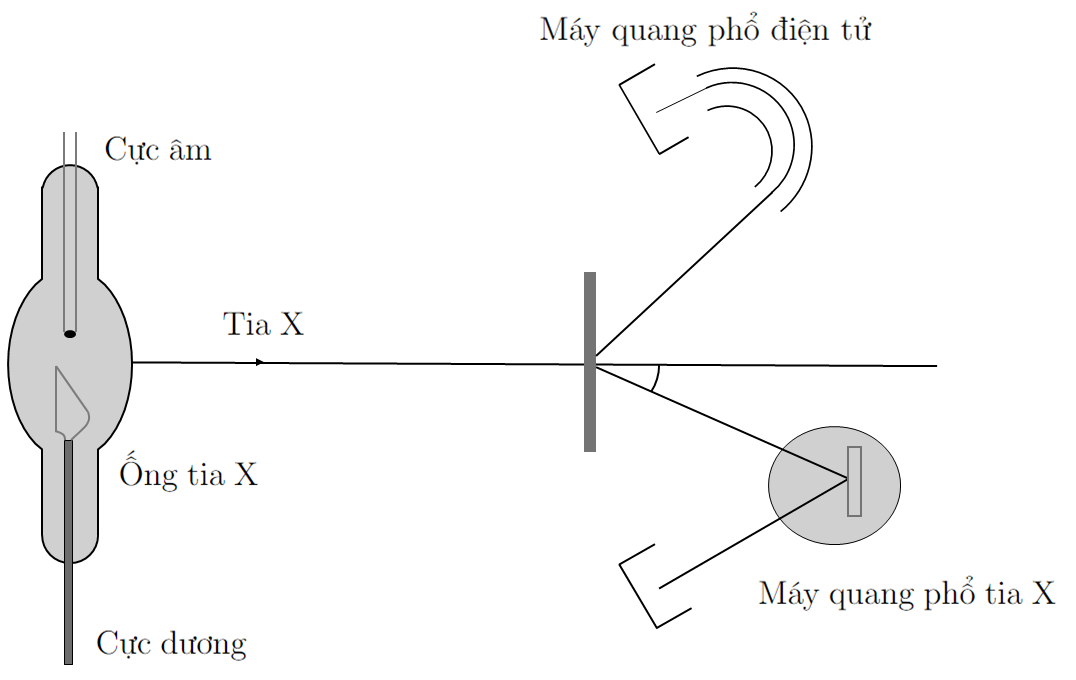
\includegraphics[width=0.65\textwidth]{images/Hinh 8a.png}
  \begin{center}
    \figurename{ 8a: Sơ đồ bố trí thí nghiệm.}
  \end{center}
\end{figure}

\begin{figure}[h]
  \centering
  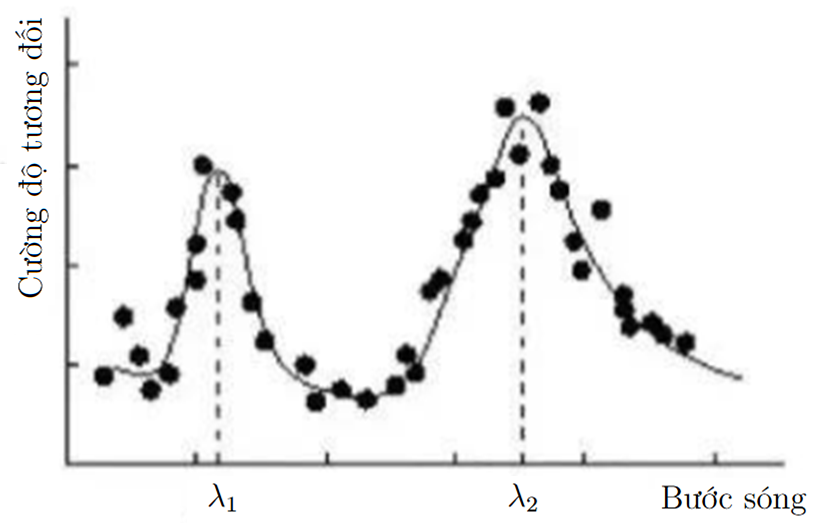
\includegraphics[width=0.58\textwidth]{images/Hinh 8b.png}
  \begin{center}
    \figurename{ 8b: Quang phổ tia X.}
  \end{center}
\end{figure}

\noindent Biết hằng số Rydberg $R_{\infty}=$\SI{10973731}{\metre^{-1}}, $hc=$\SI{1240}{\nano\metre\electronvolt} trong đó $h$ và $c$ lần lượt là hằng số Plank và vận tốc ánh sáng trong chân không.
\begin{enumerate}
  \item Lý thuyết Bohr có thể lý giải các mức năng lượng và phổ của nguyên tử Hydrogen hoặc hệ ion hoá giống Hydrogen. Năng lượng và trạng thái của electron trong hệ phụ thuộc vào số lượng tử $n$. Đối với hệ nguyên tử gồm nhiều electron, electron trong nguyên tử có thể được chia thành các lớp vỏ $K(n=1), L(n=2)$ và $M(n=3)$ tuỳ thuộc vào giá trị của $n$. BIết rằng năng lượng của electron trong lớp $K$ của nguyên tử kim loại ở anode là \SI{-20,1}{\kilo\electronvolt}.
        \begin{enumerate}
          \item[a.] Xác định điện áp tối thiểu cần sử dụng để ion hoá một electron trong lớp vỏ $K$ của nguyên tử kim loại, từ đó gây ra sự chuyển dịch mức năng lượng của electron từ lớp $L$ về lớp $K$ và phát ra tia X. Kết quả làm tròn đến ba chữ số thập phân.
          \item[b.] Với điện áp tính được ở ý a, bước sóng ngắn nhất của tia X phán ra từ ống tia X là bao nhiêu? Kết quả làm tròn đến ba chữ số thập phân.
          \item[c.] Nếu năng lượng của photon tia X đặc trưng $K_{\alpha}$ phát ra từ nguyên tử kim loại là \SI{17,44}{\kilo\electronvolt}, hãy xác định số điện tích hạt nhân của nguyên tử này.
        \end{enumerate}
  \item Sử dụng tia X đặc trưng $K_{\alpha}$ có bước sóng $\lambda$ tác động vào một bia vật liệu, giả sử electron trong bia vật liệu ở trạng thái tĩnh và có khối lượng nghỉ là $m$. Biết góc tán xạ (góc giữa tia X tán xạ và tia X tới) là $\theta$. Hãy tìm bước sóng của tia X tán xạ và động năng của electron quang điện tử.
  \item Trong thí nghiệm, phổ tán xạ đo được tại góc $\theta=135^{\circ}$. Hình 8b cho thấy có hai đỉnh phổ ứng với các bước sóng $\lambda_{1}$ và $\lambda_{2}$. Giải thích nguồn gốc hai đỉnh phổ này và nguyên nhân khiến cho độ rộng của đỉnh phổ $\lambda_{1}$ lớn hơn độ rộng của đỉnh phổ $\lambda_{2}$.
\end{enumerate}

\newpage

%%%%%%%%%% TITLE#2 %%%%%%%%%%
\begin{center}
  \noindent\Large\textbf{LỜI GIẢI THAM KHẢO}
\end{center}
\vspace{5mm}

%%%%%%%%%% SOLUTIONS %%%%%%%%%%
\setcounter{equation}{0}
\noindent\textbf{Câu I:}\\
\noindent\textbf{1a.}
\begin{equation*}
  M=\frac{\pi r^{2}L}{2}(1+c)
\end{equation*}
\begin{equation*}
  d=\frac{\dfrac{\pi r^{2}L}{2}\left(\dfrac{4r}{3\pi}-\dfrac{4r}{3\pi}c\right)}{\dfrac{\pi r^{2}L}{2}(1+c)}=\frac{4r}{3\pi}\left(\frac{1-c}{1+c}\right)
\end{equation*}

\noindent\textbf{1b.} Momen quán tính của một khối trụ đặc có khối lượng $M$ và bán kính $r$ là $\dfrac{1}{2}Mr^2$ do đó
\begin{equation*}
  I=\frac{1}{2}\left(\frac{\pi r^{2}L}{2}\right)(1+c)r^{2}=\frac{\pi r^{4}L}{4}(1+c)
\end{equation*}

\noindent\textbf{2.} Định luật II Newton cho
\begin{equation*}
  \tau=I\ddot{\theta}
\end{equation*}
momen lực đối với trục đối xứng là
\begin{equation*}
  \begin{gathered}
    \tau=-Mgd\sin\theta \\
    I\ddot{\theta}=-Mgd\sin\theta \\
    \ddot{\theta}=-\frac{Mgd}{I}\sin\theta \\
    \Rightarrow T=\frac{2\pi}{\omega}=2\pi\sqrt{\frac{I}{Mgd}}
  \end{gathered}
\end{equation*}

\noindent\textbf{3a.} \\
\noindent\underline{\textbf{Cách 1}}: Phương trình chuyển động của khối trụ đối với trục quay đi qua điểm tiếp xúc
\begin{equation*}
  \tau=I_{\text{con}}\ddot{\theta}
\end{equation*}
momen lực tác dụng lên khối trụ tương tự như ý trên
\begin{equation*}
  \tau = -Mgd\sin\theta\approx - M g d \theta
\end{equation*}
momen quán tính đối với trục quay qua điểm tiếp xúc được cho bởi
\begin{equation*}
  I_{\text{con}}=I_{cm}+M(r-d)^{2}
\end{equation*}
\begin{equation*}
  I=I_{cm}+Md^{2}
\end{equation*}
\begin{equation*}
  \Rightarrow I_{\text{con}}=I+M((r-d)^{2}-d^{2})=I+M(r^{2}-2rd)
\end{equation*}
\begin{equation*}
  \Rightarrow\ddot{\theta}=-\frac{Mgd}{I_{con}}\theta
\end{equation*}
chu kì dao động
\begin{equation*}
  T=2\pi\sqrt{\frac{I_{con}}{Mgd}}=2\pi\sqrt{\frac{I+M(r^{2}-2rd)}{Mgd}}
\end{equation*}
có thể thấy, khi $d\rightarrow0$, chu kì $T\rightarrow0$.\\

\noindent\underline{\textbf{Cách 2}}: Hàm Lagrange là
\begin{equation*}
  L=T-U=\frac{1}{2}I_{con}\dot{\theta}^2-\frac{1}{2}Mgd\theta^2
\end{equation*}
phương trình chuyển động được cho bởi
\begin{equation*}
  \begin{gathered}
    \frac{d}{dt}\frac{\partial L}{\partial\theta}-\frac{\partial L}{\partial\theta}=0\Rightarrow I_{con}\ddot{\theta}+Mgd\theta=0 \\
    \Rightarrow\ddot{\theta}=-\frac{Mgd}{I_{con}}\theta                                                                           \\
    \Rightarrow T=2\pi\sqrt{\frac{I_{con}}{Mgd}}=2\pi\sqrt{\frac{I+M(r^{2}-2rd)}{Mgd}}
  \end{gathered}
\end{equation*}

\noindent\textbf{3b.} Vì khối trụ chỉ có thể lăn không trượt, năng lượng của nó là bảo toàn. Để thoát khỏi sự dao động, khối trụ phải có đủ động năng để khối tâm có thể lên đến vị trí thế năng cực đại
\begin{equation*}
  \frac{1}{2}Mv_{cm}^{2}+\frac{1}{2}I_{cm}\omega_{0}^{2}+Mg(r-d)=Mg(r+d)
\end{equation*}
\begin{equation*}
  \begin{gathered}
    \Rightarrow\frac{1}{2}M\omega_{0}^{2}(r-d)^{2}+\frac{1}{2}(I-Md^{2})\omega_{0}^{2}=2Mgd \\
    \Rightarrow\omega_{0}=\sqrt{\frac{4Mgd}{M(r-d)^{2}+(I-Md^{2})}}
  \end{gathered}
\end{equation*}
có thể thấy, khi $d\rightarrow0$, $\omega_0\rightarrow0$, điều này có nghĩa không có bất kì cân bằng bền nào trong giới hạn này và khối trụ sẽ tiếp tục di chuyển về một phía.\\

\newpage
\setcounter{equation}{0}
\noindent\textbf{Câu II:}\\
\noindent\textbf{1.1}
\begin{equation*}
  m = \rho V = \rho \cdot \left(\frac{\pi d^2}{4} \cdot h\right) = 9{,}6 \times 10^{-4}~\text{kg}
\end{equation*}

\noindent\textbf{1.2} Moment từ của nam châm có thể được tính thông qua định nghĩa của độ từ hóa:
\begin{equation*}
  M_R = \frac{p_m}{V} \quad \implies \quad p_m = M_R V
\end{equation*}
Sử dụng mối liên hệ đã cho giữa độ từ hóa và cảm ứng từ dư $B_R = \mu_0 M_R$, ta thu được:
\begin{equation*}
  p_m = \frac{B_R}{\mu_0} \cdot \left( \frac{\pi d^2}{4} \cdot h \right) = 0{,}14~\text{Am}^2
\end{equation*}

\noindent\textbf{1.3} Cường độ dòng điện từ hoá có thể được tính theo công thức moment từ:
\begin{equation*}
  p_m = I_m S \implies I_m = \frac{p_m}{S} = \left( \frac{B_R}{\mu_0} \right) \cdot \left( \frac{V}{S} \right) = \frac{B_R}{\mu_0} h = 1{,}1 \times 10^4~\text{A}
\end{equation*}

\noindent\textbf{2.1} Các thành phần của cảm ứng từ do từ tích điểm gây ra được xác định từ công thức:

\begin{equation*}
  B = \frac{\mu_0}{4\pi}\frac{q_m}{R^2}
\end{equation*}
kết hợp với hình vẽ ta được:
\begin{figure}[H]
  \centering
  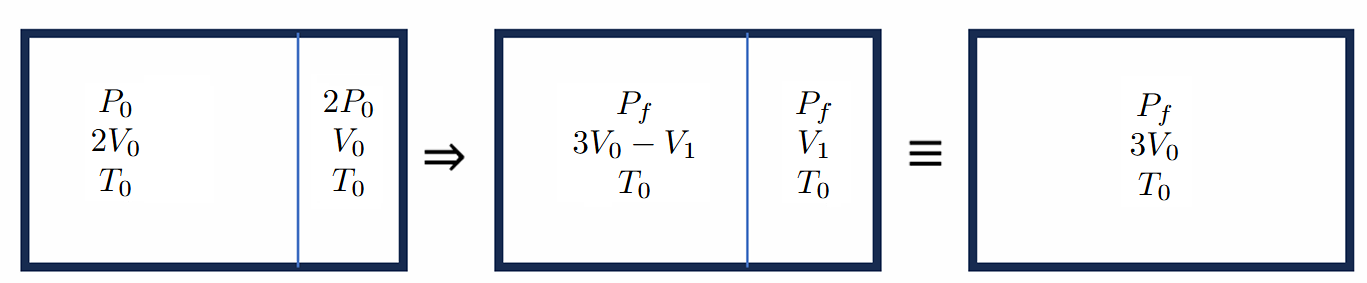
\includegraphics[width=0.2\textwidth]{Figures/Solutions/Fig 2.1.png}
\end{figure}

\begin{equation*}
  B^{(0)}_z(r, z)  = \frac{\mu_0}{4\pi}\frac{q_m}{R^2} \cos \alpha = \frac{\mu_0 q_m}{4\pi} \frac{z}{(r^2 + z^2)^{3/2}} \\
\end{equation*}
\begin{equation*}
  B^{(0)}_r(r, z)  = \frac{\mu_0}{4\pi}\frac{q_m}{R^2} \sin \alpha = \frac{\mu_0 q_m}{4\pi} \frac{r}{(r^2 + z^2)^{3/2}}
\end{equation*}

\noindent\textbf{2.2}\\
\begin{figure}[H]
  \centering
  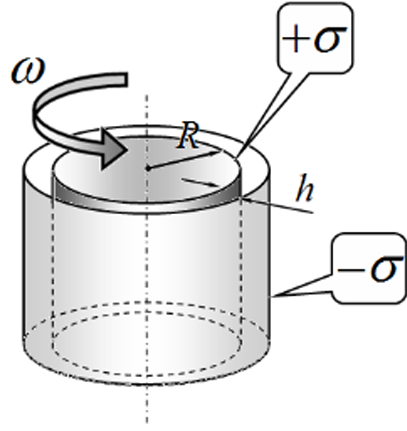
\includegraphics[width=0.3\textwidth]{Figures/Solutions/Fig 2.2.png}
\end{figure}

\noindent\textbf{2.3} Để giải phần này, ta có thể dùng gợi ý trong đề. Cách thứ hai là dùng nguyên lý chồng chất, viết biểu thức chính xác cho cảm ứng từ và khai triển theo tham số nhỏ $a$. Ở đây, ta sẽ sử dụng cách ngắn gọn hơn:
\begin{equation*}
  B_z(r, z) = B^{(0)}_z(r, z) - B^{(0)}_z(r, z + a) \approx -\left(B^{(0)}_z(r, z)\right)' \cdot a    \\
\end{equation*}
\begin{equation*}
  B_z(r, z)  = -\frac{\mu_0 q_m a}{4\pi} \cdot \frac{d}{dz} \left[ \frac{z}{(r^2 + z^2)^{3/2}} \right]  = \frac{\mu_0 p_m}{4\pi} \frac{2z^2 - r^2}{(r^2 + z^2)^{5/2}}
\end{equation*}

\noindent\textbf{2.4} Đồ thị định tính của hàm này có thể được vẽ thông qua các phân tích định tính: hàm là chẵn, bằng 0 tại $r = \pm \sqrt{2}z$, có các đoạn đơn điệu rõ ràng, tiệm cận về 0 khi $z \to \pm\infty$.\\
\begin{figure}[H]
  \centering
  \begin{subfigure}[b]{0.49\textwidth}
    \centering
    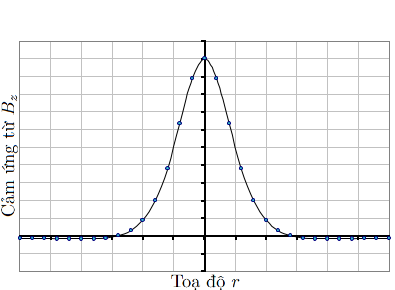
\includegraphics[width=0.9\textwidth]{Figures/Solutions/Fig 2.3.png}
  \end{subfigure}
  \hfill
  \begin{subfigure}[b]{0.49\textwidth}
    \centering
    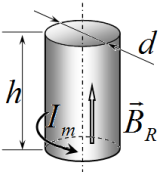
\includegraphics[width=0.6\textwidth]{Figures/Solutions/Fig 2.4.png}
  \end{subfigure}
\end{figure}


\noindent\textbf{2.5} Với $r = 0$ ta có:
\begin{equation*}
  B_z(z) = \frac{\mu_0 p_m}{4\pi} \frac{2z^2 - r^2}{(r^2 + z^2)^{5/2}} \Big|_{r = 0} = \frac{\mu_0 p_m}{2\pi z^3}
\end{equation*}

\noindent\textbf{2.6} Thực hiện tương tự:
\begin{equation*}
  B_r(r, z) = B^{(0)}_r(r, z) - B^{(0)}_r(r, z + a) = -\left(B^{(0)}_r(r, z)\right)' \cdot a
\end{equation*}
\begin{equation*}
  B_r(r, z) = -\frac{\mu_0 q_m a}{4\pi}  \left[ \frac{r}{(r^2 + z^2)^{3/2}} \right]'
  = \frac{\mu_0 p_m}{4\pi} \frac{3rz}{(r^2 + z^2)^{5/2}}
\end{equation*}

\noindent\textbf{2.7} Đồ thị của hàm này có thể được xây dựng trên cơ sở các phân tích định tính: hàm là lẻ, bằng 0 tại $z = 0$; có xu tiệm cận về 0 khi $z \to \pm \infty$.\\
\begin{figure}[H]
  \centering
  \begin{subfigure}[b]{0.49\textwidth}
    \centering
    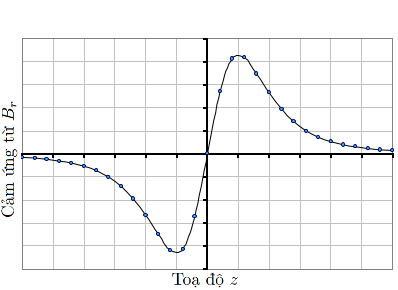
\includegraphics[width=0.9\textwidth]{Figures/Solutions/Fig 2.5.png}
  \end{subfigure}
  \hfill
  \begin{subfigure}[b]{0.49\textwidth}
    \centering
    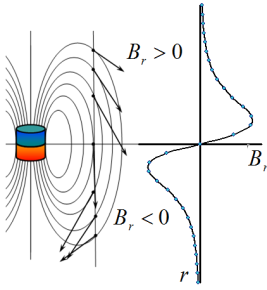
\includegraphics[width=0.6\textwidth]{Figures/Solutions/Fig 2.6.png}
  \end{subfigure}
\end{figure}


\noindent\textbf{2.8} Cảm ứng từ theo phương $r$ là cực đại khi:
\begin{equation*}
  \left(B_r(r, z)\right)'_z  = \frac{\mu_0 p_m}{4\pi}  3r \left( \frac{z}{(r^2 + z^2)^{5/2}} \right)'  = \frac{\mu_0 p_m}{4\pi}  3r  \frac{r^2 - 4z^2}{(r^2 + z^2)^{7/2}} = 0
\end{equation*}
Từ phương trình trên suy ra vị trí cực trị là $z^* = \pm \dfrac{r}{2}$. Giá trị cực đại là:
\begin{equation*}
  B_{r\text{max}}(r, z) = \frac{\mu_0 p_m}{4\pi} \frac{3rz}{(z^2 + r^2)^{5/2}} \Big|_{z = \frac{r}{2}}  = \frac{3}{2} \left( \frac{4}{5} \right)^{5/2} \frac{\mu_0 p_m}{4\pi r^3} = C  \frac{\mu_0 p_m}{r^3}
\end{equation*}
Trong đó:
\begin{equation*}
  C = \frac{3}{8\pi} \left( \frac{4}{5} \right)^{5/2} \approx 0{,}068
\end{equation*}

\begin{wrapfigure}[7]{r}{5.5cm}
  \centering
  \vspace{-0.5cm}
  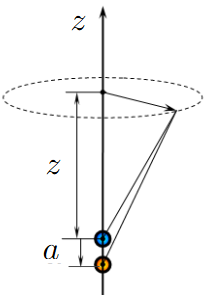
\includegraphics[width=0.28\textwidth]{Figures/Solutions/Fig 2.7.png}
\end{wrapfigure}
\noindent\textbf{3.1} Xét một lưỡng cực từ nằm trong một từ trường không đều $B(z)$. Hướng của moment lưỡng cực song song với hướng của trường từ. Khi đó, tổng lực tác dụng lên lưỡng cực là:
\begin{equation*}
  F = -q_m B(z) + q_m B(z + a)
\end{equation*}
Vì $a \ll z$, biểu thức có thể viết lại dưới dạng:
\begin{equation*}
  F \approx q_m a \cdot \frac{B(z + a) - B(z)}{a} = p_m B'(z)
\end{equation*}
Trong đó $B'(z)$ là đạo hàm của cảm ứng từ theo $z$. Ta có:
\begin{equation*}
  F = p_m \cdot \frac{d}{dz} \left( \frac{\mu_0 p_m}{2\pi z^3} \right) = -\frac{3\mu_0 p_m^2}{2\pi z^4}
\end{equation*}

\noindent\textbf{3.2} Với cách sắp xếp nam châm như trong hình a), lực từ cân bằng với trọng lực:
\begin{equation*}
  \frac{3\mu_0 p_m^2}{2\pi L^4} = mg
\end{equation*}
Từ đó suy ra khoảng cách cần tìm:
\begin{equation*}
  L = \left( \frac{3 \mu_0 p_m^2}{2\pi m g} \right)^{1/4}
\end{equation*}

\noindent\textbf{3.3} Chỉ có thể thực hiện thí nghiệm với phương án a), vì trạng thái cân bằng trong trường hợp này là bền. Cân bằng trong trường hợp b) là không bền.\\

\noindent\textbf{3.4} Thay giá trị số ta thu được:
\begin{equation*}
  L = 3{,}3~\text{cm}
\end{equation*}

\begin{wrapfigure}[11]{r}{5.5cm}
  \centering
  \vspace{-0.5cm}
  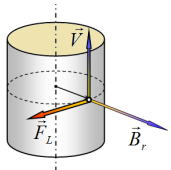
\includegraphics[width=0.28\textwidth]{Figures/Solutions/Fig 2.8.png}
\end{wrapfigure}
\noindent\textbf{4.1} Khi nam châm chuyển động, từ trường tại mỗi điểm trên thành ống sẽ biến thiên, từ đó sinh ra dòng điện cảm ứng, còn gọi là dòng Foucault.\\
\indent Để thuận tiện cho việc tính toán, ta sẽ sử dụng hệ quy chiếu gắn với nam châm. Trong hệ quy chiếu này, ống nhôm chuyển động trong từ trường. Nguồn của suất điện động (EMF) là lực Lorentz tác dụng lên điện tích dưới ảnh hưởng của thành phần xuyên tâm $B_r$ của cảm ứng từ. Lực Lorentz có phương này tiếp tuyến với thành ống và có độ lớn:
\begin{equation*}
  F_L = q V B_r
\end{equation*}
Suất điện động xuất hiện trong vòng dây ôm lấy ống là:
\begin{equation*}
  \varepsilon = \frac{1}{q} F_L \cdot 2\pi r_0 = 2\pi r_0 B_r V
\end{equation*}
Áp dụng định luật Ohm ta có:
\begin{equation*}
  \Delta I = \frac{\varepsilon}{R} = \frac{B_r V h_0 \Delta z}{\rho}
\end{equation*}
Cuối cùng:
\begin{equation*}
  \Delta I = \frac{B_{r,\text{max}} V h_0 \Delta z}{\rho}
\end{equation*}

\begin{wrapfigure}[7]{r}{4.5cm}
  \centering
  \vspace{-0.5cm}\hspace{-1cm}
  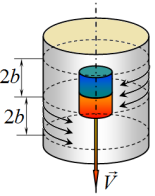
\includegraphics[width=0.2\textwidth]{Figures/Solutions/Fig 2.9.png}
\end{wrapfigure}
\noindent\textbf{4.2} Dòng điện xuất hiện ở tất cả các phần của ống nơi tồn tại từ trường xuyên tâm. Trong mô hình gần đúng “bậc thang”, thành phần xuyên tâm tồn tại trong một vùng có chiều rộng $4b$. Hướng của dòng điện không quan trọng vì công suất nhiệt không phụ thuộc vào hướng dòng. Vì vậy, ta có thể dùng biểu thức cho cường độ dòng điện hiệu dụng:
\begin{equation*}
  I = \frac{B_{r,\text{max}} V h_0}{\rho} \cdot 4b
\end{equation*}
Công suất toả nhiệt có thể được xác định thông qua định luật Joule–Lenz:
\begin{equation*}
  P = I^2 R
\end{equation*}
Trong đó $R = \rho \cdot \frac{2\pi r_0}{4b h_0}$ là điện trở phần thành ống nơi dòng điện chạy qua. Như vậy:
\begin{equation*}
  P = \left( \frac{B_{r,\text{max}} V h_0}{\rho} \cdot ab \right)^2 \cdot \frac{2\pi r_0}{4b h_0}   = \left( \frac{8\pi r_0 b h_0}{\rho} \right) B_{r,\text{max}}^2 V^2
\end{equation*}

\noindent\textbf{4.3} Công suất nhiệt tính được ở trên chính là công do lực ma sát từ sinh ra:
\begin{equation*}
  P = F \cdot V
\end{equation*}
Do đó, lực ma sát từ có độ lớn:
\begin{equation*}
  F = \left( \frac{8\pi r_0 b h_0}{\rho} \right) B_{r,\text{max}}^2 V
\end{equation*}

\noindent\textbf{4.4} Vận tốc của nam châm ổn định khi lực ma sát từ bằng với trọng lượng của nam châm:
\begin{equation*}
  \left( \frac{8\pi r_0 b h_0}{\rho} \right) B_{r,\text{max}}^2 V = mg \implies V = \frac{mg \rho}{8\pi r_0 b h_0 B_{r,\text{max}}^2}
\end{equation*}

\noindent\textbf{4.5}
\begin{equation*}
  B_{r,\text{max}} = C \frac{\mu_0 p_m}{r_0^3} \approx 0{,}45~\text{T}
\end{equation*}
\begin{equation*}
  V = \frac{mg \rho}{8\pi r_0 b h_0 B_{r,\text{max}}^2} \approx 3{,}9~\text{cm/s}
\end{equation*}




\newpage
\setcounter{equation}{0}
\noindent\textbf{Câu III:}\\
\subsection*{Phần 1: Giới thiệu Toán học}
\noindent\textbf{1.} Để chứng minh công thức \eqref{eq:p31} ta cần sử dụng các phép xấp xỉ cho hàm mũ:
\begin{equation}
  \label{eq:31}
  \sqrt{a^{2} + x^{2}} = a \left( 1 + \frac{x^{2}}{a^{2}} \right)^{1/2} \approx a \left( 1 + \frac{x^{2}}{2a^{2}} \right) = a + \frac{x^{2}}{2a}
\end{equation}

\noindent\textbf{2.} Phương trình của đường tròn được mô tả có dạng:
\begin{equation}
  \label{eq:32}
  x^{2} + (y - R)^{2} = R^{2}
\end{equation}
sử dụng công thức \eqref{eq:p31} trong đề bài ta được:
\begin{equation}
  \label{eq:33}
  x^{2} + (y - R)^{2} = R^{2} \implies y - R = \pm \sqrt{R^{2} - x^{2}} \implies y = R - \frac{x^{2}}{2R}
\end{equation}

\subsection*{Phần 2: Sự đẳng thời}
\begin{wrapfigure}[11]{r}{6cm}
  \centering
  \vspace{-4mm}
  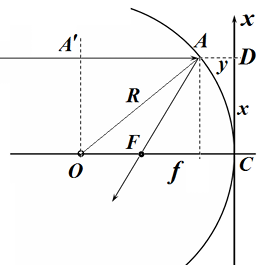
\includegraphics[width=0.3\textwidth]{Figures/P3/Fig 3.1S.png}
\end{wrapfigure}

\noindent\textbf{1.} Ta có thể xem tiêu điểm là ảnh của một điểm sáng nằm tại vô cùng. Theo nguyên lý đẳng thời cho sự  tạo ảnh, ta cần chứng minh rằng tồn tại một điểm $F$ mà  thời gian ánh sáng chuyển động đến $F$ là như nhau với mọi tia sáng. Do tính đối xứng, điểm này phải nằm trên quang trục. Trong trường hợp này ánh sáng truyền đi trong môi trường đồng nhất, nên để thời gian truyền là bằng nhau, chiều dài các đường truyền phải bằng nhau. Lấy một tia bất kỳ $AA' $ song song với quang trục , cách quang trục một đoạn $x=CD$. Vì các tia tới là song song, khoảng cách từ điểm vật ở vô cùng đến bất kỳ mặt phẳng nào vuông góc với các tia (và trục quang học chính) là như nhau. Để đơn giản, chọn mặt phẳng $A'O $, đi qua tâm hình học của gương. Khi đó, điều kiện đẳng thời có thể được phát biểu như sau: phải tồn tại một điểm $F$ sao cho khoảng cách $ AF + A'F = l $ không phụ thuộc vào $ x $. Từ hình vẽ, khoảng cách này được biểu diễn qua các tham số của hệ dưới dạng:
\begin{equation}
  \label{eq:34}
  l = f + \sqrt{(R - y)^{2} + x^{2}} = (R - y) + \sqrt{f^{2} + x^{2}}
\end{equation}
trong đó $ y = AD $; $ f = CF $ là tiêu cự của gương (nếu tiêu điểm tồn tại). Bây giờ, ta cần tìm một hàm $ y = f(x) $ sao cho biểu thức trên luôn thỏa mãn với mọi $ x $. Thực hiện các biến đổi đại số đơn giản, ta có:
\begin{equation}
  \label{eq:35}
  \sqrt{x^{2} + (f-y)^{2} } = y + f \implies x^{2}+f^{2}-2yf+y^{2}=y^{2}+2yf+f^{2}\implies 4yf=x^{2}
\end{equation}
tức bề mặt của gương là một đường parabol:
\begin{equation}
  \label{eq:36}
  y = \frac{x^{2}}{4f}
\end{equation}
thì tất cả các tia song song với trục quang học sẽ đến điểm $ F $ cùng một lúc, do đó điểm này sẽ là tiêu điểm.
Nói cách khác, nếu gương có dạng parabol, các tia luôn hội tụ tại $F$. Như đã chỉ ra, đối với các tia bàng trục, cung tròn có thể xem như một đoạn parabol, hay có thể phát biểu ngược lại: parabol có thể được thay thế bằng cung tròn. Ta có:
\begin{equation}
  \label{eq:37}
  y = \frac{x^{2}}{2R} \quad \text{thì} \quad f = \frac{R}{2}
\end{equation}
tiêu cự gương cầu:
\begin{equation}
  \label{eq:38}
  f = \frac{R}{2}
\end{equation}

\begin{wrapfigure}[11]{r}{8cm}
  \centering
  \vspace{-4mm}
  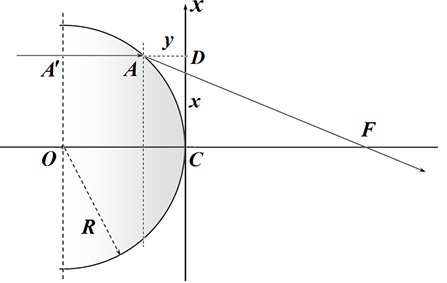
\includegraphics[width=0.45\textwidth]{Figures/P3/Fig 3.2S.png}
\end{wrapfigure}

\noindent\textbf{2.} Lập luận tương tự ý trước điều kiện tồn tại của tiêu điểm là: thời gian mà ánh sáng đi qua khoảng cách $AF + A'A$ không phụ thuộc vào khoảng cách $x$ từ tia sáng đến quang trục. Giả sử ánh sáng truyền đi một khoảng cách $ l $ trong môi trường đồng nhất có chiết suất $ n $, khi đó thời gian truyền bằng:
\begin{equation}
  \label{eq:39}
  t = \frac{l}{c/n} = \frac{nl}{c}
\end{equation}
với $c/n $ là tốc độ ánh sáng trong môi trường này. Lưu ý rằng thay vì tính toán sự thay đổi của tốc độ ánh sáng (điều thực sự xảy ra), khi tính toán thời gian truyền, ta có thể coi tốc độ ánh sáng không đổi (và bằng tốc độ ánh sáng trong chân không $ c $) nhưng độ dài đường truyền tăng lên thành $ nl $ (trong quang học, đại lượng này được gọi là độ dài đường đi quang học). Do đó, điều kiện tồn tại của tiêu điểm là đẳng thức sau được thỏa mãn với mọi giá trị của $ x $:
\begin{equation}
  \label{eq:310}
  n(R-y)+\sqrt{x^{2}+(f+y)^{2}}=nR+f
\end{equation}
biến đổi ta được:
\begin{equation}
  \label{eq:311}
  \sqrt{x^{2}+(f+y)^{2}}=f+ny\implies x^{2}+f^{2}+2fy+y^{2}=f^{2}+2fny+n^{2}y^{2}\implies x^{2}=2(n-1)fy
\end{equation}
nếu mặt cong của thấu kính được mô tả bằng phương trình:
\begin{equation}
  \label{eq:312}
  y = \frac{x^{2}}{2(n - 1)f}
\end{equation}
thì đẳng thức \eqref{eq:310} sẽ được thỏa mãn với mọi giá trị của $ x $, tức $ F $ là tiêu điểm. Nhưng hàm này mô tả trong xấp xỉ paraxial một "cung tròn" có bán kính $ R $:
\begin{equation}
  \label{eq:313}
  y = \frac{x^{2}}{2R}
\end{equation}
do đó, thấu kính được mô tả trong điều kiện bài toán có tiêu điểm. Để xác định tiêu cự của thấu kính, ta chỉ cần so sánh các biểu thức \eqref{eq:312} và \eqref{eq:313}, từ đó suy ra rằng tiêu cự này bằng:
\begin{equation}
  \label{eq:314}
  f = \frac{R}{n-1}
\end{equation}

\begin{wrapfigure}[10]{r}{8cm}
  \centering
  \vspace{-8mm}
  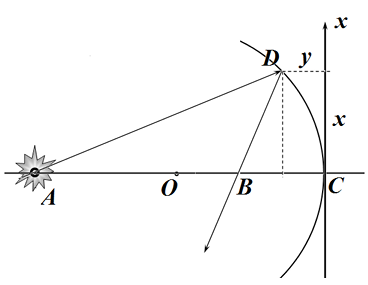
\includegraphics[width=0.4\textwidth]{Figures/P3/Fig 3.3S.png}
\end{wrapfigure}

\noindent\textbf{3a.} Tương tự như các bài toán trước: để tồn tại ảnh tại điểm $B$, khoảng cách $ DB + AD $ không phụ thuộc vào vị trí của điểm $ D $ trên bề mặt gương và bằng khoảng cách $ CB + AC $. Điều kiện này sẽ được thỏa mãn nếu đẳng thức:
\begin{equation}
  \label{eq:315}
  \sqrt{x^{2}+(a-y)^{2}}+\sqrt{x^{2}+(b-y)^{2}}=a+b
\end{equation}
được thỏa mãn với mọi $ x $. Bình phương tổng của các căn thức là một bài toán không đơn giản, vì vậy chúng ta sẽ sử dụng các công thức gần đúng để biến đổi đẳng thức \eqref{eq:315}. Trước tiên, ta sẽ viết lại \eqref{eq:315} dưới dạng:
\begin{equation}
  \label{eq:316}
  \sqrt{x^{2}+(a-y)^{2}}+\sqrt{x^{2}+(b-y)^{2}}\approx \sqrt{x^{2}+a^{2}-2ay}+\sqrt{x^{2}+b^{2}-2by}
\end{equation}
ở đây, ta đã bỏ qua các số hạng $ y^{2} $, nhưng giữ lại các số hạng $ x^{2} $. Trước đó, ta đã chỉ ra rằng đối với đường tròn (và tiếp tuyến parabol), đại lượng $ y $ tỷ lệ với $ x^{2} $, vì vậy các đại lượng này là các số hạng nhỏ cùng bậc. Đại lượng $ y^{2} $ tỷ lệ với $ x^{4} $, do đó có thể bỏ qua nó. Sử dụng mối quan hệ giữa các đại lượng nhỏ này, chúng ta tiếp tục các biến đổi đại số, sử dụng công thức \eqref{eq:p31} được cho trong đề bài:
\begin{equation}
  \label{eq:317}
  \sqrt{x^{2}+a^{2}-2ay}+\sqrt{x^{2}+b^[2]-2by}\approx a+\frac{(x^{2}-2ay)}{2a}+b+\frac{(x^{2}-2by)}{2a}
\end{equation}
thay vào \eqref{eq:315}:
\begin{equation}
  \label{eq:318}
  a+\frac{(x^{2}-2ay)}{2a}+b+\frac{(x^{2}-2by)}{2a}=a+b
\end{equation}
từ đó suy ra rằng \eqref{eq:315} sẽ được thỏa mãn với nếu hàm $ y(x) $ có dạng như sau:
\begin{equation}
  \label{eq:319}
  y=\frac{x^{2}}{4a}+\frac{x^{2}}{4b}=\left(\frac{1}{a}+\frac{1}{b}\right)\frac{x^{2}}{4}
\end{equation}
một lần nữa, chúng ta nhận được phương trình của parabol, có thể coi như parabol tiếp tuyến với đường tròn. So sánh biểu thức \eqref{eq:319} với phương trình "parabol" của đường tròn:
\begin{equation*}
  y = \frac{x^{2}}{2R}
\end{equation*}
ta có thể nhận thấy rằng tồn tại một giá trị $ b $, mà đẳng thức (15) được thỏa mãn với mọi tia sáng phát ra từ điểm $ A $. Nghĩa là ảnh của điểm này tồn tại.\\

\noindent\textbf{3b.} Từ \eqref{eq:319} và phương trình "đường tròn", ta có công thức gương cần tìm:
\begin{equation}
  \frac{1}{a}+\frac{1}{b}=\frac{2}{R}=\frac{1}{f}
\end{equation}
ở đây, ta đã sử dụng giá trị tiêu cự đã nhận được trước đó $ f = \dfrac{R}{2} $.\\

\noindent\textbf{4a.} Trong trường hợp này, các tia sáng xuất phát từ điểm $A$ và phản xạ từ gương sẽ không giao nhau. Nhưng chúng có thể giao nhau tại một điểm kéo dài của các tia phản xạ. Giả sử rằng để kéo dài các tia, khoảng cách phải được coi là âm. \\

\begin{wrapfigure}[10]{r}{8cm}
  \centering
  \vspace{-8mm}
  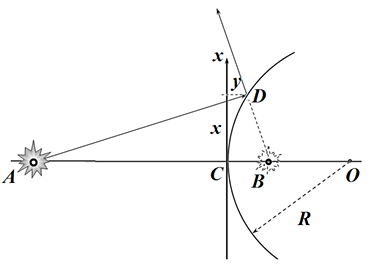
\includegraphics[width=0.42\textwidth]{Figures/P3/Fig 3.4S.png}
\end{wrapfigure}

\noindent\textbf{4b.} Trong khuôn khổ giả định này, điều kiện tồn tại của ảnh ảo được phát biểu như sau: khoảng cách $DB-AD$ là như nhau đối với tất cả các tia phản xạ từ gương, và bằng $CB-AC=b-a$. Điều kiện này được viết dưới dạng đẳng thức, tương tự như (15):
\setcounter{equation}{19}
\begin{equation}
  \label{eq:320}
  \sqrt{x^{2}+(a+y)^{2}}-\sqrt{x^{2}+(b-y)^{2}}=a-b
\end{equation}
biến đổi ta được:
\begin{align}
  \label{eq:321}
   & \sqrt{x^{2}+(a+y)^{2}}-\sqrt{x^{2}+(b-y)^{2}}\approx\sqrt{x^{2}+a^{2}+2ay}-\sqrt{x^{2}+b^{2}-2by}                                 \\
   & \approx \left(a+\frac{x^{2}+2ay}{2a}\right)-\left(b+\frac{x^{2}-2by}{2b}\right)=a-b\implies\frac{x^{2}}{2a}-\frac{x^{2}}{ab}+2y=0
\end{align}
sử dụng "phương trình parabol" của đường tròn:
\begin{equation*}
  y=\frac{x^{2}}{2R}
\end{equation*}
ta có:
\begin{equation}
  \label{eq:322}
  \frac{1}{a}-\frac{1}{b}=-\frac{2}{R}
\end{equation}
công thức này tương tự với "công thức gương cầu lõm" nếu:
\begin{itemize}
  \item Khoảng cách đến ảnh ảo là âm;
  \item Tiêu cự cũng phải là âm $f=-\frac{R}{2}$.
\end{itemize}

\noindent\textbf{4c.} Quang học hình học là một xấp xỉ của quang học sóng. Do đó, nguyên lý đẳng thời có thể được giải thích như sau:
\begin{itemize}
  \item Mỗi tia sáng có thể tương ứng với một sóng nào đó;
  \item  Nếu tất cả các sóng này đi từ nguồn đến ảnh trong cùng một thời gian, thì các pha của chúng là giống nhau;
  \item  Kết quả là tại điểm ảnh sẽ xảy ra sự giao thoa với cường độ tối đa.
\end{itemize}

\subsection*{Phần 3: Nguyên lý Fermat}
\begin{wrapfigure}[6]{r}{8cm}
  \centering
  \vspace{-12mm}
  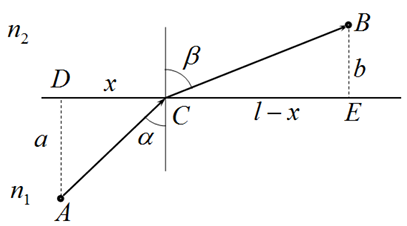
\includegraphics[width=0.4\textwidth]{Figures/P3/Fig 3.5S.png}
\end{wrapfigure}

\noindent\textbf{1.} Giả sử tia sáng đi từ điểm $A$ đến điểm $B$ (xem hình), khúc xạ tại ranh giới giữa hai môi trường tại điểm $C$. Vị trí của điểm này được xác định bởi khoảng cách $x$ tính từ điểm $D$. Đặt $DE=l$, khi đó $CE=l-x$. Thời gian di chuyển của ánh sáng theo đường $ACB$ bằng:
\begin{equation}
  \label{eq:323}
  \tau(x)=\frac{\sqrt{a^{2}+x^{2}}}{c/n_{1}}+\frac{\sqrt{b^{2}+(l-x)^{2}}}{c/n_{2}}=\frac{n_{1}\sqrt{a^{2}+x^{2}}+n_{2}\sqrt{b^{2}+(l-x)^{2}}}{c}
\end{equation}
theo nguyên lý Fermat, khi di chuyển theo quỹ đạo thực, thời gian này là nhỏ nhất, tức ta phải tìm cực trị của hàm \eqref{eq:323}
\begin{equation}
  \label{eq:324}
  \tau'(x)=\frac{2n_{1}x}{2\sqrt{a^{2}+x^{2}}}-\frac{2n_{2}(l-x)}{2\sqrt{b^{2}+(l-x)^{2}}}=0
\end{equation}
từ hình vẽ, ta có:
\begin{equation}
  \label{eq:325}
  \sin{\alpha}=\frac{x}{\sqrt{a^{2}+x^{2}}}, \quad \sin{\beta}=\frac{l-x}{\sqrt{b^{2}+(l-x)^{2}}}
\end{equation}
do đó, từ \eqref{eq:324} và \eqref{eq:325}, suy ra định luật khúc xạ ánh sáng:
\begin{equation}
  \label{eq:326}
  n_{1}\sin{\alpha}=n_{2}\sin{\beta}
\end{equation}

\begin{wrapfigure}[5]{r}{5.5cm}
  \centering
  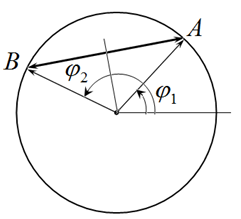
\includegraphics[width=0.25\textwidth]{Figures/P3/Fig 3.6S.png}
\end{wrapfigure}

\noindent\textbf{2a.} Để tính độ dài của quỹ đạo, ta sẽ sử dụng công thức đơn giản cho độ dài dây cung $l$ của $AB$, được viết tổng quát như sau:
\begin{equation}
  \label{eq:327}
  l=2R\lvert\sin\frac{\varphi_{1}-\varphi_{2}}{2}\rvert
\end{equation}
\begin{figure}[h]
  \centering
  \vspace{1cm}
  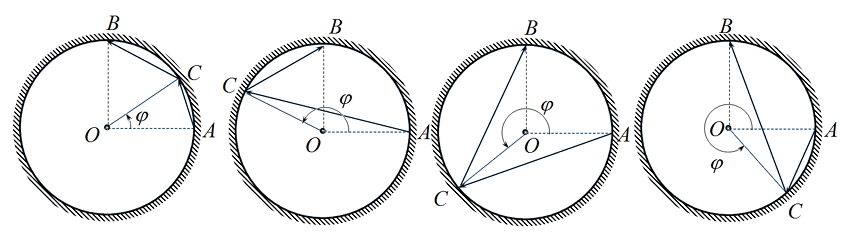
\includegraphics[width=1\textwidth]{Figures/P3/Fig 3.7S.png}
\end{figure}

\noindent độ dài quỹ đạo tia sáng với một lần phản xạ từ bề mặt trong $ACB$ bằng tổng độ dài của hai dây cung, do đó có thể được mô tả bằng công thức:
\begin{equation}
  \label{eq:328}
  L=2R\left(\sin\frac{\varphi}{2}+\lvert\sin\left(\frac{\varphi}{2}-\frac{\pi}{4}\right)\rvert\right)
\end{equation}
viết lại công thức này cho hai khoảng giá trị của góc $\phi$, khi $\phi \leqslant \dfrac{\pi}{2}$:
\begin{equation}
  \label{eq:329}
  L=2R\sin\frac{\varphi}{2}+2R\sin\frac{\pi/2-\varphi}{2}=4R\sin\frac{\pi}{8}\cos\left(\frac{\pi}{8}-\frac{\varphi}{2}\right)
\end{equation}
khi $\varphi\geqslant\dfrac{\pi}{2}$:
\begin{equation}
  \label{eq:330}
  L=2R\sin\frac{\varphi}{2}+2R\sin\frac{\varphi-\pi/2}{2}=4R\sin\left(\frac{\varphi}{2}-\frac{\pi}{8}\right)\cos\left(\frac{\pi}{8}\right)
\end{equation}

\noindent Đồ thị biểu diễn sự phụ thuộc này được chỉ ra trên hình:
\begin{figure}[h]
  \centering
  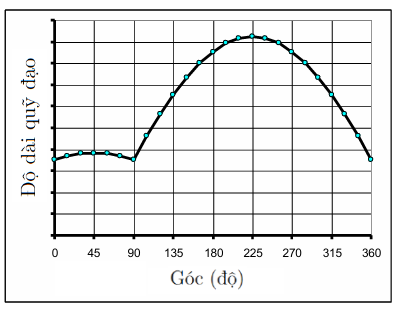
\includegraphics[width=0.6\textwidth]{Figures/P3/Fig 3.8S.png}
\end{figure}

\noindent\textbf{2b.} Các quỹ đạo thực của tia sáng thỏa mãn định luật phản xạ ánh sáng xảy ra khi:
\begin{equation}
  \label{eq:331}
  \varphi=\begin{cases}
    \dfrac{\pi}{4} \\
    \dfrac{\pi}{4}+\pi=\dfrac{5\pi}{4}
  \end{cases}
\end{equation}
với các giá trị này, độ dài của quỹ đạo là tối đa.\\

\noindent\textbf{3a.} Nguyên lý Fermat có thể được hiểu như sau: ánh sáng chọn từ nhiều con đường giữa hai điểm ra một con đường đòi hỏi thời gian cực trị (tối thiểu hoặc tối đa) hoặc thời gian tĩnh (không phụ thuộc vào quỹ đạo). Về mặt toán học, nguyên lý này được phát biểu như sau: Giả sử chiều dài của quỹ đạo được mô tả bởi một hàm số của tham số $\xi$, xác định quỹ đạo, $L(\xi)$. Khi đó, các quỹ đạo thực tương ứng với các giá trị tham số $\xi^*$, mà tại đó đạo hàm của hàm số bằng không:
\begin{equation}
  \label{eq:332}
  L'(\xi^*)=0
\end{equation}

\noindent\textbf{3b.} Giải thích nguyên lý Fermat xuất phát từ tính chất sóng của ánh sáng. Trong phạm vi lân cận điểm cực trị, khi tham số thay đổi từ giá trị tĩnh $\xi^*$ một lượng nhỏ $\Delta\xi$, chiều dài của quỹ đạo sẽ thay đổi một lượng tỉ lệ với $(\Delta\xi)^2$. Do đó, gần điểm cực trị có một phạm vi rộng của các quỹ đạo mà chiều dài của chúng thay đổi một lượng rất nhỏ. Các sóng lan truyền dọc theo những quỹ đạo này đến điểm quan sát với độ lệch pha, do đó thỏa mãn điều kiện cực đại của giao thoa.
























\newpage
\setcounter{equation}{0}
\noindent\textbf{Câu IV:}\\
\noindent\textbf{1.} Như được chỉ ra trên hình 4.1, góc vì $\sin\alpha=\dfrac{1}{2}$ nên $\alpha=30^\circ$. Theo định luật khúc xạ ánh sáng
\begin{equation*}
  \sin\beta=\frac{\sin\alpha}{n}=\frac{1}{2n}\Rightarrow\tan\beta=\frac{1}{\sqrt{4n^{2}-1}}
\end{equation*}
từ hình vẽ, dễ dàng nhận thấy
\begin{equation*}
  \begin{gathered}
    x_{0}=\frac{R}{2}-\frac{\sqrt{3}}{2}R\tan\gamma \\
    \tan\gamma=\tan(\alpha-\beta)=\frac{\tan\alpha-\tan\beta}{1+\tan\alpha\tan\beta}=\frac{\sqrt{4n^{2}-1}-\sqrt{3}}{\sqrt{12n^{2}-3}+1} \\
    x_{0}=\frac{R}{2}\left(1-\frac{\sqrt{12n^{2}-3}-3}{\sqrt{12n^{2}-3}+1}\right)=\frac{2R}{\sqrt{12n^{2}-3}+1}
  \end{gathered}
\end{equation*}

\noindent\textbf{2.} Tại thời điểm $t$, mặt tiếp xúc sẽ có dạng một hình tròn bán kính $r$. Trong thời gian $dt$ tiếp theo, nhiệt lượng truyền vào khối băng là
\begin{equation*}
  \mathrm{d}Q=K\pi r^{2}dt
\end{equation*}
với $K$ là hằng số. Thể tích băng nóng chảy là
\begin{equation*}
  dQ=Ldm=L\rho\pi r^{2}dz
\end{equation*}
với $L$ và $\rho$ tương ứng là ẩn nhiệt chuyển pha và khối lượng riêng của băng. Như vậy ta có
\begin{equation*}
  K\pi r^{2}dt=-L\rho\pi r^{2}dz
\end{equation*}
\begin{equation*}
  \Rightarrow\frac{dz}{dt}=-\frac{K}{L\rho}=\text{const}
\end{equation*}
do đó
\begin{equation*}
  z(t)=R\left(1-\frac{t}{T_0}\right)
\end{equation*}

\begin{figure}[h]
  \centering
  \begin{subfigure}[b]{0.49\textwidth}
    \centering
    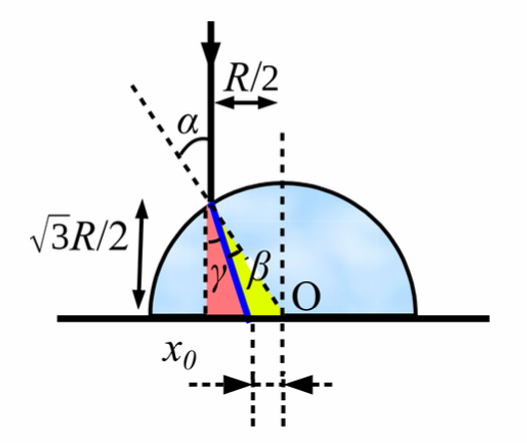
\includegraphics[width=0.95\textwidth]{Figures/Solutions/Fig 4.1.png}
    \begin{center}
      \figurename{ 4.1}
    \end{center}
  \end{subfigure}
  \hfill
  \begin{subfigure}[b]{0.49\textwidth}
    \centering
    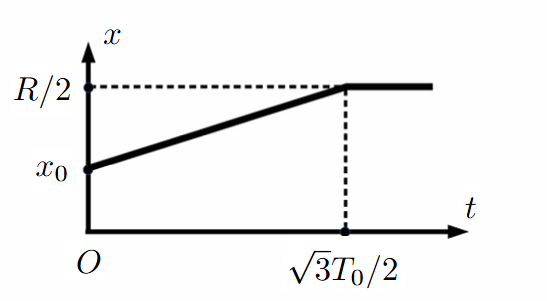
\includegraphics[width=0.95\textwidth]{Figures/Solutions/Fig 4.2.png}
    \begin{center}
      \figurename{ 4.2}
    \end{center}
  \end{subfigure}
\end{figure}

\noindent\textbf{3.} Khi bán kính của khối băng nhỏ hơn hoặc bằng $\dfrac{R}{2}$, chùm laser sẽ chiếu thẳng xuống bàn, tức $x(t)=\dfrac{R}{2}$. Khi này độ cao của khối băng là $z(t)=\left(1-\frac{\sqrt{3}}{2}\right)R$, điều này sẽ xảy ra tại $t=\dfrac{\sqrt{3}}{2}T_0$. Như vậy, với $t>\dfrac{\sqrt{3}}{2}T_0$, ta có $x(t)=\dfrac{R}{2}$.\\
\noindent Với $t<\dfrac{\sqrt{3}}{2}T_0$, ta sẽ sử dụng các tam giác đồng dạng
\begin{equation*}
  \begin{gathered}
    \frac{\frac{R}{2}-x_{0}}{\frac{R}{2}-x(t)}=\frac{\frac{\sqrt{3}}{2}R}{R\left(\frac{\sqrt{3}}{2}-\frac{t}{T_{0}}\right)} \\
    \Rightarrow\left(\frac{R}{2}-x_{0}\right)\left(\frac{\sqrt{3}}{2}-\frac{t}{T_{0}}\right)=\frac{\sqrt{3}}{2}\left(\frac{R}{2}-x\right) \\
    \Rightarrow x(t)=\frac{R}{2}-\left(\frac{R}{2}-x_{0}\right)\left(1-\frac{2}{\sqrt{3}}\frac{t}{T_{0}}\right)=\frac{R}{2}-\frac{R}{2}\left(1-\frac{4}{\sqrt{12n^{2}-3}+1}\right)\left(1-\frac{2}{\sqrt{3}}\frac{t}{T_{0}}\right)
  \end{gathered}
\end{equation*}

\newpage
\setcounter{equation}{0}
\noindent\textbf{Câu V:}\\
\noindent\textbf{1.} Khi hạt chuyển động tròn đều trong mặt phẳng vuông góc với trục $Oz$, nó không chịu tác dụng của lực nào trên phương $Oz$, do đó:
\begin{equation}
  \label{eq:51}
  \hat{z}\cdot e\vec{E}=\frac{ep}{4\pi\varepsilon_{0}r_{0}^{3}}(3\cos^{2}\theta_{0}-1)=0
\end{equation}
suy ra:
\begin{equation}
  \label{eq:52}
  \cos\theta_{0}=\pm\frac{\sqrt{3}}{3}
\end{equation}
và vì hạt chuyển động tròn, lực tác dụng lên nó trong mặt phẳng $Oxy$ phải có phương hướng tâm. Phương trình \eqref{eq:52} chỉ có hai nghiệm, đó là:
\begin{equation}
  \label{eq:53}
  F=\frac{-3ep}{4\pi\varepsilon_{0}r_{0}^{3}}\cos\theta_{0}\sin\theta_{0}>0
\end{equation}
trong phương trình \eqref{eq:52} chỉ có một nghiệm thoả mãn yêu cầu $\cos\theta_{0}<0$, tức là ta có:
\begin{equation}
  \label{eq:54}
  \cos\theta_{0}=-\frac{\sqrt{3}}{3} \implies \theta_{0}=\pi-\arccos\frac{\sqrt{3}}{3}
\end{equation}
bán kính quỹ đạo của hạt là $R=r_{0}\sin\theta_{0}$, thay \eqref{eq:53} vào phương trình của định luật II Newton:

\begin{equation}
  \label{eq:55}
  F=m\frac{v_{0}^{2}}{R}
\end{equation}
ta có:
\begin{equation*}
  v_{0}=\sqrt{\frac{FR}{m}}=\sqrt{-\frac{3eq}{4\pi\varepsilon_{0}mr_{0}^{2}}\cos\theta_{0}\sin^{2}\theta_{0}}=\sqrt{-\frac{3eq}{4\pi\varepsilon_{0}r_{0}^{2}}\cos\theta_{0}(1-\cos^{2}\theta_{0})}
\end{equation*}
sử dụng \eqref{eq:54} ta được:
\begin{equation}
  \label{eq:56}
  v_{0}=\sqrt{\frac{\sqrt{3}eq}{6\pi\varepsilon_{0}mr_{0}^{2}}}
\end{equation}

\noindent\text{2a.} Momen động lượng của hạt là:
\begin{equation}
  \label{eq:57}
  \vec{L}=\vec{r}\times m \vec{v}=\vec{r}\times m(\dot{r}\hat{r}+r\dot{\theta}\hat{\theta})=mr^{2}\dot{\theta}\hat{n}
\end{equation}
momen lực tác dụng lên hạt:
\begin{equation}
  \label{eq:58}
  \tau=\vec{r}\times e\vec{E}=-\frac{e}{4\pi\varepsilon_{0}r^{3}}\vec{r}\times\vec{p}=\frac{ep\sin\theta}{4\pi\varepsilon_{0}r^{2}}\hat{n}
\end{equation}
với $\hat{n}=\hat{r}\times\hat{\theta}$. Phương trình chuyển động của hạt:
\begin{equation}
  \label{eq:59}
  \frac{dL}{dt}=\frac{d(mr^{2}\dot{\theta})}{dt}=\frac{ep\sin\theta}{4\pi\varepsilon_{0}r^{2}}
\end{equation}
nhân vế theo vế phương trình \eqref{eq:59} với $L=mr^{2}\dot{\theta}$ ta được:
\begin{equation*}
  L\frac{dL}{dt}=\frac{ep\sin\theta}{4\pi\varepsilon_{0}r^{2}}\cdot mr^{2}\frac{d\theta}{dt}=\frac{mep\sin\theta}{5\pi\varepsilon_{0}}\frac{d\theta}{dt}
\end{equation*}
điều này dẫn tới:
\begin{equation*}
  \frac{dL^{2}}{dt}=-\frac{d}{dt}\left(\frac{mep}{2\pi\varepsilon_{0}}\cos\theta\right)
\end{equation*}
suy ra:
\begin{equation}
  \label{eq:510}
  L^{2}+\frac{mep}{2\pi\varepsilon_{0}}\cos\theta=\text{const}
\end{equation}
hạt đứng yên tại $t=0$, nghĩa là:
\begin{equation}
  \label{eq:511}
  L^{2}=\frac{mep}{2\pi\varepsilon_{0}}(\cos\theta_{0}-\cos\theta)
\end{equation}

\noindent\textbf{2b.} Điện thế do lưỡng cực điện tạo ra:
\begin{equation*}
  \varphi=\frac{\vec{p}\cdot\vec{r}}{4\pi\varepsilon_{0}r^{3}}=\frac{p\cos\theta}{4\pi\varepsilon_{0}r^{2}}
\end{equation*}
bảo toàn năng lượng:
\begin{equation}
  \label{eq:512}
  \frac{1}{2}mv^{2}+e\varphi=\frac{1}{2}m(\dot{r}^{2}+r^{2}\dot{\theta}^{2})+\frac{ep\cos\theta}{4\pi\varepsilon_{0}r^{2}}=\frac{ep\cos\theta_{0}}{4\pi\varepsilon_{0}r_{0}^{2}}
\end{equation}
hay dưới dạng động lượng $p_{r}=mv_{r}$ và momen động lượng $L=mr^{2}\dot{\theta}$:
\begin{equation}
  \label{eq:513}
  \frac{p_{r}^{2}}{2m}+\frac{L^{2}}{2mr^{2}}+\frac{ep\cos\theta}{4\pi\varepsilon_{0}r^{2}}=\frac{ep\cos\theta_{0}}{4\pi\varepsilon_{0}r_{0}^{2}}
\end{equation}
thay \eqref{eq:511} vào \eqref{eq:513} ta được:
\begin{equation*}
  v_{r}^{2}=\frac{ep\cos\theta_{0}}{2\pi m\varepsilon_{0}}\left(\frac{1}{r_{0}^{2}}-\frac{1}{r^{2}}\right)
\end{equation*}
suy ra:
\begin{equation}
  \label{eq:514}
  v_{r}=\sqrt{\frac{ep\cos\theta_{0}}{2\pi m\varepsilon_{0}}\left(\frac{1}{r_{0}^{2}-\frac{1}{r^{2}}}\right)}
\end{equation}

\noindent\textbf{2c.} Vì $v_{r}^{2}\geqslant 0$ nên từ \eqref{eq:514} ta có:
\begin{equation*}
  \text{khi}\theta_{0}<\frac{\pi}{2}, r\geqslant r_{0}
\end{equation*}
lúc này, $v_{r}=\dot{r}=\sqrt{\dfrac{ep\cos\theta_{0}}{2\pi m\varepsilon_{0}}\left(\dfrac{1}{r_{0}^{2}}-\dfrac{1}{r^{2}}\right)}$ tăng khi $r$ tăng. Chuyển động của hạt không bị giới hạn.
\begin{equation*}
  \text{khi}\theta_{0}>\frac{\pi}{2}, r\leqslant r_{0}
\end{equation*}
\begin{equation*}
  \text{khi}\theta_{0}=\frac{\pi}{2}, r=r_{0}
\end{equation*}
trong cả hai trường hợp trên, chuyển động của hạt đều bị giới hạn. Do đó, điều kiện cần tìm là:
\begin{equation}
  \label{eq:515}
  \theta_{0}\geqslant\frac{\pi}{2}
\end{equation}
nếu $\theta_{0}=\dfrac{pi}{2}$, chuyển động của hạt bị giới hạn hoàn toàn, $v_{r}=\dot{r}=0$. Khoảng cách từ hạt đến gốc toạ độ không đổi trong suốt quá trình chuyển động và bằng $r_{0}$; và vì $L\geqslant 0$, phương trình \eqref{eq:511} đòi hỏi:
\begin{equation}
  \label{eq:516}
  L^{2}=-\frac{mep}{2\pi\varepsilon_{0}}\cos\theta\geqslant 0
\end{equation}
như vậy, chuyển động của hạt thoả mãn
\begin{equation}
  \label{eq:517}
  r=r_{0}, \cos\theta\leqslant 0
\end{equation}
có thể thấy, quỹ đạo của nó là một đường bán nguyệt có bán kính $r_{0}$ $\left(\dfrac{\pi}{2}\leqslant\theta\leqslant\dfrac{3\pi}{2}\right)$ trong mặt phẳng thẳng đứng.

\noindent\textbf{2d.} Trong trường hợp chuyển động của hạt không bị giới hạn, phương trình \eqref{eq:514} có thể được viết lại dưới dạng:
\begin{equation}
  \label{eq:518}
  \frac{dr}{dt}=\sqrt{\frac{ep\cos\theta_{0}}{2\pi\varepsilon_{0}m}\left(\frac{1}{r_{0}^{2}}-\frac{1}{r^{2}}\right)}
\end{equation}
hay:
\begin{equation*}
  \sqrt{\frac{ep\cos\theta_{0}}{2\pi\varepsilon_{0}mr_{0}^{2}}dt=\frac{rdr}{\sqrt{r^{2}-r_{0}^{2}}}=d\sqrt{r^{2}-r_{0}^{2}}}
\end{equation*}
qua đó:
\begin{equation}
  \label{eq:519}
  \sqrt{r^{2}-r_{0}^{2}}-\sqrt{\frac{ep\cos\theta_{0}}{2\pi\varepsilon_{0}mr_{0}^{2}}}t=\text{const}
\end{equation}
sử dụng điều kiện bao đầu $r(t=0)=r_{0}>0$, ta có:
\begin{equation*}
  \sqrt{r^{2}-r_{0}^{2}}-\sqrt{\frac{ep\cos\theta_{0}}{2\pi\varepsilon_{0}mr_{0}^{2}}}t=0
\end{equation*}
suy ra:
\begin{equation}
  \label{eq:520}
  r=\sqrt{r_{0}^{2}+\frac{ep\cos\theta_{0}}{2\pi\varepsilon_{0}mr_{0}^{2}}t^{2}}
\end{equation}

\newpage
\setcounter{equation}{0}
\noindent\textbf{Câu VI:}\\
\noindent\textbf{1.} Từ trường bên ngoài quả cầu là:
\begin{equation}
  \label{eq:61}
  \vec{B}=\vec{B}_{e}+\vec{B}'=\vec{B}_{e}+\frac{\mu_{0}}{4\pi r^{3}}\left[3(\vec{m}\cdot\hat{r})\hat{r}-\vec{m}\right]
\end{equation}
đối với một vật dẫn lý tưởng, từ trương bên trong nó bằng không, mặt khác, theo định lý Gauss cho từ trường, thành phân theo phương pháp tuyến của từ trường là liên tục, do đó:
\begin{equation}
  \label{eq:62}
  \hat{r}\cdot\vec{B}\vert_{r=a}=\hat{r}\cdot\vec{B}_{e}+\frac{\mu_{0}}{2\pi a^{3}}(\vec{m}\cdot\hat{r})=0
\end{equation}
do tính đối xứng, $\vec{m}$ phải song song hoặc phản song song với $\vec{B}_{e}$, theo đó, từ \eqref{eq:62} ta có:
\begin{equation}
  \label{eq:63}
  \vec{m}=-\frac{2\pi a^{3}}{\mu_{0}}\vec{B}_{e}
\end{equation}
từ trường  bên ngoài là chồng chập của trường được tạo ra từ dòng điện từ hoá trên quả cầu (tương tự với từ trường tạo ra bởi lưỡng cực từ $\vec{m}$) và từ trường ngoài $\vec{B}_{e}$. Thay \eqref{eq:63} vào \eqref{eq:61} ta được:
\begin{equation}
  \label{eq:64}
  \vec{B}=\vec{B}_{e}-\frac{a^{3}}{2r^{3}}\left[3(\vec{B}_{e}\cdot\hat{r})\hat{r}-\vec{B}_{e}\right]
\end{equation}
theo định lý Ampere, mật độ dòng điện trên bề mặt quả cầu được cho bởi:
\begin{equation}
  \label{eq:65}
  \mu\vec{i}=\hat{r}\times\vec{B}\vert_{r=a}
\end{equation}
thay \eqref{eq:64} vào \eqref{eq:65} ta được:
\begin{equation}
  \label{eq:66}
  \vec{i}=\hat{r}\times\frac{3\vec{B}_{e}}{2\mu_{0}}=\left(-\frac{3B_{e}}{2\mu_{0}\sin\theta}\right)\hat{\phi}
\end{equation}

\noindent\textbf{2.} Do tính đối xứng, cảm ứng từ do dòng điện trong dây dẫn tạo ra tại một điểm nằm trên trục đối xứng của nó có hướng dọc theo trục $Oz$. Sử dụng định luật Biot-Savart-Laplace, ta có:
\begin{equation*}
  \vec{B}=\frac{\mu_{0}I}{4\pi(b^{2}+h^{2})}\frac{b}{\sqrt{b^{2}+h^{2}}}2\pi b\hat{z}
\end{equation*}
hay:
\begin{equation}
  \label{eq:67}
  \vec{B}=\left[\frac{\mu_{0}I_{0}b^{2}}{2(b^{2}+h^{2})^{3/2}}\cos\omega t\right]\hat{z}=B_{0}\cos\omega t\hat{z}
\end{equation}
trong đó:
\begin{equation*}
  B_{0}=\frac{\mu_{0}I_{0}b^{2}}{2(b^{2}+h^{2})^{3/2}}
\end{equation*}

\noindent\textbf{3.} Vì $a\ll b$ nên từ trường do vòng dây tạo ra ở khu vực gần quả cầu dẫn gần như là đều, xấp xỉ từ trường tại tâm quả cầu, được cho bởi phương trình \eqref{eq:67}. Và vì $b\ll a$, quả cầu dẫn có thể xem là lý tưởng và momen lưỡng cực từ của nó có thể tìm được từ phương trình \eqref{eq:63}:
\begin{equation}
  \label{eq:68}
  \vec{m}=-\frac{2\pi a^{3}}{\mu_{0}}\vec{B}
\end{equation}
vì $\vec{m}$ và $\vec{B}$ đều hướng dọc theo trục $Oz$ nên lực tác dụng lên quả cầu là:
\begin{equation*}
  \vec{F}(t)=m\frac{dB}{dz}\hat{z}
\end{equation*}
do đó:
\begin{equation*}
  \vec{F}=-\frac{2\pi a^{3}}{\mu_{0}}B\frac{dB}{dz}\hat{z}=-\frac{\pi a^{3}}{\mu_{0}}\frac{dB^{2}}{dz}\hat{z}
\end{equation*}
thay \eqref{eq:67} vào ta được:
\begin{equation}
  \label{eq:69}
  \vec{F}(t)=-\frac{\pi a^{3}}{\mu_{0}}\frac{d}{dz}\left[\frac{\mu_{0}^{2}I_{0}^{2}b^{4}}{4(b^{2}+z^{2})^{3}}\cos^{2}\omega t\right]=\frac{3\pi a^{3}b^{4}z}{2(b^{2}+z^{2})^{4}}\mu_{0}I_{0}^{2}\cos^{2}\omega t\hat{z}
\end{equation}
mặt khác:
\begin{equation*}
  \langle \cos^{2}\omega t \rangle=\frac{1}{2\pi/\omega}\int_{0}^{2\pi/\omega}\cos^{2}\omega tdt=\frac{1}{2}
\end{equation*}
do đó:
\begin{equation}
  \label{eq:610}
  \langle F \rangle=\frac{1}{2\pi/\omega}\int_{0}^{2\pi/\omega}\vec{F}dt=\frac{3\pi a^{3}b^{4}h}{4(b^{2}+h^{2})^{4}}\mu_{0}I_{0}^{2}\hat{z}
\end{equation}
phương trình cân bằng:
\begin{equation}
  \label{eq:611}
  \langle F \rangle = G
\end{equation}
từ đây ta tìm được:
\begin{equation}
  \label{eq:611}
  I_{0}=\sqrt{\frac{4G(b^{2}+h^{2})^{4}}{3\pi a^{3}b^{4}\mu_{0} h}}
\end{equation}

\noindent\textbf{4.} Thay \eqref{eq:66} vào \eqref{eq:67} ta tìm được  mật đồ dòng điện bề mặt gần đúng trên quả cầu dẫn. Do đó, mật độ dòng điện trong bề dày đặc trưng của quả cầu là:
\begin{equation}
  \label{eq:613}
  \vec{J}=\frac{\vec{i}}{\delta}=\left(-\frac{3B}{2\mu_{0}\delta}\sin\theta\right)\hat{\phi}
\end{equation}
theo định luật Joule, mật độ công suất nhiệt là:
\begin{equation}
  \label{eq:614}
  p=\frac{J^{2}}{\sigma}=\frac{9B^{2}}{4\mu_{0}^{2}\sigma\delta^{2}}\sin^{2}\theta
\end{equation}
do đó, tổng công suất toả nhiệt là:
\begin{equation}
  \label{eq:615}
  P(t)=\int pdV=\int p 2\pi r^{2}\sin\theta drd\theta=\frac{9\pi B^{2}}{2\mu_{0}^{2}\sigma \delta^{2}}\int_{a-\delta}^{a}r^{2}dr\int_{0}^{\pi}\sin^{3}\theta d\theta
\end{equation}
trong đó:
\begin{equation}
  \label{eq:616}
  \int_{a-\delta}^{a}r^{2}dr=\frac{1}{3}[a^{3}-(a-\delta)^{3}]\approx a^{2}\delta
\end{equation}
và:
\begin{equation}
  \label{eq:617}
  \int_{0}^{\pi}\sin^{3}\theta d\theta=\int_{-1}^{1}(1-\cos^{2}\theta)d\cos\theta=\frac{4}{3}
\end{equation}
do đó:
\begin{equation}
  \label{eq:618}
  P(t)=6\pi a^{2}\frac{B^{2}}{\mu_{0}^{2}\sigma\delta}
\end{equation}
thay \eqref{eq:67} và $\delta=\sqrt{\dfrac{2}{\omega\mu_{0}\sigma}}$ vào \eqref{eq:618} ta được:
\begin{equation}
  \label{eq:619}
  P(t)=\frac{3}{4}\frac{\pi a^{2}b^{4}I_{0}^{2}}{(b^{2}+h^{2})^{3}}\sqrt{\frac{2\omega\mu_{0}}{\sigma}}\cos^{2}\omega t
\end{equation}
vì vậy, công suất toả nhiệt trung bình là:
\begin{equation}
  \label{eq:620}
  \langle P \rangle = \frac{3}{8}\frac{\pi a^{2}b^{4}I_{0}^{2}}{(b^{2}+h^{2})^{3}}\sqrt{\frac{2\omega\mu_{0}}{\sigma}}
\end{equation}



\newpage
\setcounter{equation}{0}
\noindent\textbf{Câu VII:}\\
\begin{wrapfigure}[13]{r}{10cm}
  \centering
  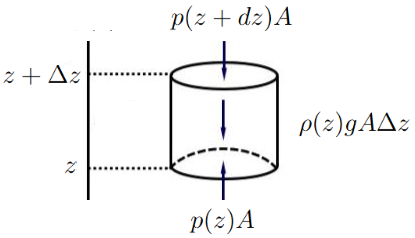
\includegraphics[width=0.5\textwidth]{images/Hinh 7a (S).png}
  \begin{center}
    \figurename{ 7a}
  \end{center}
\end{wrapfigure}

\noindent\textbf{1.} Ở độ cao $z$, áp suất khí quyển là $p(z)$, nhiệt độ là $T(z)$, sử dụng phương trình trạng thái khí lý tưởng, ta tìm được khối lượng riêng của không khí là:
\begin{equation}
  \label{eq:71}
  \rho(z)=\frac{n\mu}{V}=\frac{p{z}\mu}{RT(z)}
\end{equation}
trong đó $n$ là số mol, $V$ là thể tích của khí. Như trong hình 7a, trọng lượng của khí nằm trong một hình trụ bán kính đáy $A$, chiều cao $\Delta z$ ở độ cao $z$ là $\rho(z)gA\Delta z$, mặt trên của hình trụ chịu tác dụng của một lực có độ lớn $p(z+\Delta z)A$ trong khi lực tác dụng lên mặt dưới có độ lớn $p(z)A$. Vì khí bay lên từ từ, các lực tác dụng lên nó phải cân bằng với nhau:
\begin{equation}
  \label{eq:72}
  p(z+\Delta z)A+\rho(z)A\Delta zg=p(z)A
\end{equation}
cho $\Delta z\to 0$, phương trình \eqref{eq:72} có thể được viết dưới dạng:
\begin{equation}
  \label{eq:73}
  \frac{dp}{dz}=-\rho g
\end{equation}
sử dụng phương trình \eqref{eq:71}, ta được:
\begin{equation}
  \label{eq:74}
  \frac{dp}{dz}=-\frac{p\mu g}{RT}
\end{equation}
chia cả hai vế cho $p$, ta có:
\begin{equation}
  \label{eq:75}
  \frac{d\ln p}{dz}=-\frac{\mu g}{RT}
\end{equation}
trong quá trình đoạn nhiệt, $pV^{\gamma}$ là hằng số, theo phương trình trạng thái khí lý tưởng, $p^{1-\gamma}T^{\gamma}$ cũng là hằng số, tức:
\begin{equation}
  \label{eq:76}
  C=-(\gamma -1)\ln{p}+\gamma\ln{T}
\end{equation}
lấy đạo hàm hai vế phương trình \eqref{eq:76} theo $z$ ta có:
\begin{equation}
  \label{eq:77}
  0=-(\gamma - 1)\frac{d\ln p}{dz}+\gamma\frac{d\ln T}{dz}
\end{equation}
sử dụng phương trình \eqref{eq:75}:
\begin{equation}
  \label{eq:78}
  \frac{d\ln T}{dz}=\frac{1}{T}\frac{dT}{dz}=\frac{\gamma-1}{\gamma}\frac{d\ln p}{dz}=-\frac{\gamma -1}{\gamma}\frac{\mu g}{RT}
\end{equation}
vì thế:
\begin{equation}
  \label{eq:79}
  \frac{dT}{dz}=-\frac{(\gamma -1)\mu g}{\gamma R}
\end{equation}
sau khi lấy tích phân, ta nhận được:
\begin{equation}
  \label{eq:710}
  T(z)=T_{0}-\frac{(\gamma-1)\mu g}{\gamma R}z
\end{equation}

\noindent\textbf{2.} Đối với quá trình đoạn nhiệt, $pV^{\gamma}$ là hằng số, do đó ta có thể viết $p=C\rho^{\gamma}$, suy ra:
\begin{equation}
  \label{eq:711}
  v_{s}^{2}=\left(\frac{dp}{d\rho}\right)_{S}=\frac{d(C\rho^{\gamma})}{d\rho}=\gamma C\rho^{\gamma-1}=\gamma\frac{C\rho^{\gamma}}{\rho}=\gamma\frac{p}{\rho}
\end{equation}
thay $\rho=\dfrac{n\mu}{V}$ vào phương trình trạng thái khí lý tưởng $pV=nRT$ để có:

\begin{equation}
  \label{eq:712}
  v_{s}^{2}=\gamma\frac{pV}{n\mu}=\gamma\frac{nRT}{n\mu}=\gamma\frac{RT}{\mu}
\end{equation}
Do đó, ở tầng đối lưu, tốc độ truyền âm giảm khi độ cao tăng. Ở tầng bình lưu, nhiệt độ gần như không thay đổi nên tốc độ âm thanh cũng gần như không thay đổi theo độ cao; Ở tầng nghịch, nhiệt độ tăng dần theo độ cao do đó tốc độ âm thanh cũng tăng dần theo độ cao.


\noindent\textbf{3.} Trong mô hình đơn giản được giới thiệu, nhiệt độ khí bên ngoài tầng bình lưu là:
\begin{equation*}
  \SI{-10}{\degreeCelsius}=\SI{263,15}{\kelvin}
\end{equation*}
và nhiệt độ trong tầng bình lưu là:
\begin{equation*}
  \SI{-55}{\degreeCelsius}=\SI{218,15}{\kelvin}
\end{equation*}
do đó, tỉ số giữa vận tốc âm thanh bên ngoài tầng bình lưu và vận tốc âm thanh bên trong tầng bình lưu là:
\begin{equation}
  \label{eq:713}
  \frac{v_{0}}{v_{i}}=\sqrt{\frac{263,15}{218,15}}\approx 1,098
\end{equation}
khi sóng âm trong tầng bình lưu truyền đến mặt phân cách, nếu góc tới bằng $\theta_{i}$ thì theo định luật khúc xạ, góc khúc xạ $\theta_{0}$ phải thoả mãn:
\begin{equation}
  \label{eq:714}
  \sin\theta_{0}=\frac{v_{0}}{v_{i}}\sin\theta_{i}\approx 1,098\sin\theta_{i}
\end{equation}
Từ biểu thức trên, ta nhận thấy có một góc tới tới hạn:
\begin{equation}
  \label{eq:715}
  \theta_{i}^{m}=\arcsin\frac{v_{i}}{v_{0}}\approx 65,61^{\circ}
\end{equation}
khi góc tới nhỏ hơn $\theta_{i}^{m}$ thì định luật khúc xạ được thoả mãn và hiện tượng khúc xạ có thể xảy ra, khi góc tói lớn hơn $\theta_{i}^{m}$ thì định luật khúc xạ không được thoả mãn do đó sẽ xảy ra hiện tượng phản xạ toàn phần. Do đó, biểu hiện của khúc xạ và phản xạ là góc tới nhỏ hơn hay lớn hơn $\theta_{i}^{m}$. Như được biểu diễn bằng đường nét đứt trên hình 7b, khi góc tới nhỏ hơn $\theta_{i}^{m}$, sóng âm có thể phản xạ hoặc khúc xạ cùng lúc, nhờ đó âm thanh có thể được truyền vào tầng nghịch. Như được biểu diễn bằng nét liền trên hình 7b, khi góc tới lớn hơn $\theta_{i}^{m}$, sóng âm sẽ bị phản xạ toàn phần, do đó âm thanh không thể truyền vào tầng ngịch.\\

\begin{figure}[h]
  \centering
  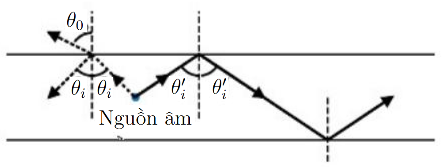
\includegraphics[width=0.53\textwidth]{images/Hinh 7b (S).png}
\end{figure}

\noindent \textbf{4.} Khi khoảng cách là tương đối lớn, ta cần xét đến hình dạng của Trái Đất. Ở đây ta có thể chia vấn đề thành 4 trường hợp, tuỳ thuộc vào vị trí của nguồn âm và đầu thu:
\begin{enumerate}
  \item[A.] Khi nguồn âm và đầu thu đều nằm trong tầng đối lưu, sẽ không có hiện tượng phản xạ toàn phần xảy ra. Vì không có hiện tượng phản xạ, đầu thu chỉ có thể thu được âm thanh nếu không bị Trái Đất cản trở, đường đi của sóng âm được biểu diễn bằng mũi tên $A$ trong hình 7c. Trong trường hợp này, khoảng cách phát hiện tối đa là:
        \begin{equation*}
          l_{1}=\sqrt{(R_{e}+h_{1})^{2}-R_{e}^{2}}\approx2\sqrt{2R_{e}h_{1}}\approx\SI{714}{\kilo\metre}
        \end{equation*}
        Vì vậy, trong trường hợp này, ta không thể phát hiện được nguồn âm ở cách xa hàng nghìn kilomet.
  \item[B.] Nguồn âm ở tầng đối lưu và đầu thu ở tầng bình lưu, do không xảy ra hiện tượng phản xạ, ta chỉ có thể thu được âm khi không bị Trái Đất cản trở, đường đi của sóng âm trong trường hợp này được biểu diễn bằng mũi tên $B$ trong hình 7c. Trong trường hợp này, khoảng cách phát hiện xa nhất sẽ không vượt quá khoảng cách từ một điểm trên đỉnh của tầng dối lưu, dọc theo tiếp tuyến của mặt phân cách đến một điểm trên đỉnh tầng bình lưu, nghĩa là nó sẽ không vượt quá:
        \begin{equation*}
          l_{1}=\sqrt{(R_{e}+h_{2})^{2}-R_{e}^{2}}-\sqrt{(R_{e}+h_{1})^{2}-R_{e}^{2}}\approx2\sqrt{2R_{e}h_{2}} + 2\sqrt{2R_{e}h_{1}}\approx\SI{862}{\kilo\metre}
        \end{equation*}
        Vì vây, trong trường hợp này, ta không thể phát hiện được nguồn âm ở cách xa hàng nghìn kilomet.
  \item[C.] Nguồn âm và đầu thu cùng ở tầng bình lưu. Vì khoảng cách giữa hai bề mặt khí quyển rất nhỏ so với bán kính Trái Đất nên sóng âm bị phản xạ toàn phần trên mặt này cũng sẽ phản xạ toàn phần trên bề mặt kia. Do đó, âm thanh có góc tới nhỏ trong tầng bình lưu có thể bị phản xạ liên tục quả hai mặt phân cách và sẽ bị giới hạn trong tầng bình lưu, do đó nó sẽ tiếp tục là truyền như được biểu diễn trên hình 7d. Vì vậy, trong trường hợp này ta có thể thu được âm thanh ở cách xa vài nghìn kilomet.
  \item[D.] Nguồn âm ở tầng bình lưu và khí cầu ở tầng đối lưu, tương tự như trường hợp $A$ và $B$, ta không thể thu được âm thanh ở cách xa vài nghìn kilomet.
\end{enumerate}

\begin{figure}[h]
  \centering
  \begin{minipage}{6cm}
    \centering
    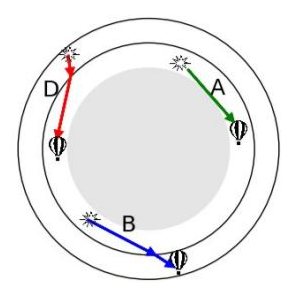
\includegraphics[width=1.1\textwidth]{images/Hinh 7c (S) .png}
    \begin{center}
      \figurename{ 7c}
    \end{center}
  \end{minipage}
  \hfil
  \begin{minipage}{6cm}
    \centering
    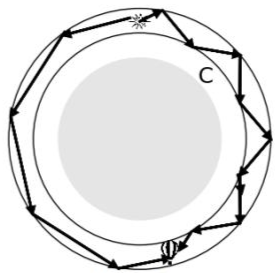
\includegraphics[width=1\textwidth]{images/Hinh 7d (S).png}
    \vspace{1mm}
    \begin{center}
      \figurename{ 7d}
    \end{center}
  \end{minipage}
\end{figure}








\newpage
\setcounter{equation}{0}
\noindent\textbf{Câu VIII:}\\
\noindent\textbf{1a.} Quá trình tạo ra tia X dòng K có thể được mô tả như sau: Electron va chạm với nguyên tử bia ở cực dương làm ion hoá một electron trong lớp K của vỏ nguyên tử bia, dẫn đến một chỗ trống trong lớp K của nguyên tử bia, electron ở lớp L ngay lập tức nhảy sang lớp K và đồng thời phát ra tia X đặc trưng $K_{\alpha}$. Giả sử động năng của các electron sinh ra ở cực âm sau khi được gia tốc bởi điện trường là:
\begin{equation}
  \label{eq:81}
  T_{e}=eU
\end{equation}
năng lượng ion hoá của các electron ở lớp K của nguyên tử bia là:
\begin{equation*}
  E_{k}=\SI{20,1}{\kilo\electronvolt}
\end{equation*}
do đó, điều kiện để một chỗ trống xuất hiện trong lớp K của nguyên tử bia là:
\begin{equation}
  \label{eq:82}
  T_{e}\geqslant E_{k}
\end{equation}
từ \eqref{eq:81} và \eqref{eq:82}, điện áp tối thiểu cần sử dụng bằng:
\begin{equation}
  \label{eq:83}
  U_{min}=\frac{E_{k}}{e}=\SI{20,1}{\kilo\electronvolt}
\end{equation}

\noindent\textbf{1b.} Tia X liên tục phát ra từ ống tia X có nguồn gốc từ bức xạ hãm do các electron va chạm với anode của tấm kim loại tạo ra. Dưới điện áp tối thiểu $U_{min}$, giả sử bước sóng ngắn nhất của tia X phát ra là $\lambda_{min}$, ta có:
\begin{equation}
  \label{eq:84}
  T_{e}h=\nu_{max}=\frac{hc}{\lambda_{min}}
\end{equation}
từ \eqref{eq:81} và \eqref{eq:84}:
\begin{equation}
  \label{eq:85}
  \lambda_{min}=\frac{hc}{eU}\approx\SI{0,0617}{\nano\metre}
\end{equation}

\noindent\textbf{8c.} Năng lượng của tia X đặc trưng $K_{\alpha}$ do nguyên tử kim loại phát ra là $E=\SI{17,44}{\kilo\electronvolt}$, nghĩa là:
\begin{equation}
  \label{eq:86}
  E=\frac{hc}{\lambda_{K\alpha}}=\SI{17,44}{\kilo\electronvolt}
\end{equation}
gọi $\lambda_{K\alpha}$ là bước sóng của tia X đặc trưng $K_{\alpha}$. Đặc điểm cấu trúc quang phổ của tia X dãy K tạo ra do sự va chạm của electron và nguyên tử bia kim loại có liên quan đến tính chất tia của nguyên tử hydrogen. Các quang phổ của hệ thống tương tự như nhau, sự khác biệt nằm ở các điện tích hạt nhân khác nhau mà electron trong nguyển tử cảm nhận được. Vì có một electron sau khi làm xuất hiện một lỗ trống trên lớp vỏ $K$ của nguyên tử bia, nên electron này có tác dụng che chắn hạt nhân. Số điện tích hạt nhân mà electron lớp $L$ cảm nhận được là một giá trị lớn hơn $Z-1$ và nhỏ hơn $Z$. Thông thường, nó được gọi là điện tích hạt nhân hiệu dụng $Z^{*}$. Theo lý thuyết Bohr, tương tự như phổ hệ thống của nguyên tử hydrogen, bước sóng của tia X đặc trưng $K_{\alpha}$ phát ra từ bia kim loại thoả mãn hệ thức:
\begin{equation}
  \label{eq:87}
  \frac{1}{\lambda_{K\alpha}}=R_{\infty}Z^{*2}\left(\frac{1}{1^{2}}-\frac{1}{2^2}\right)
\end{equation}
trong đó $R_{\infty}$ là hằng số Rydgerd và $Z^{*}$ là điện tích hạt nhân hiệu dụng. Từ \eqref{eq:86} và \eqref{eq:87} ta có:
\begin{equation}
  \label{eq:88}
  Z^{*}=\sqrt{\frac{4}{3R_{\infty}\lambda_{K\alpha}}}\sqrt{\frac{4E}{3hcR_{\infty}}}=\approx 41,35
\end{equation}
vì $Z-1<Z^{*}<Z$ nên
\begin{equation*}
  Z^{*}<Z<Z^{*}+1
\end{equation*}
từ \eqref{eq:88} ta có:
\begin{equation}
  \label{eq:89}
  Z=42
\end{equation}

\noindent\textbf{2.} Năng lượng liên kết của các electron trong bia kim loại tương đối nhỏ so với năng lượng của các photon tia X và sự tương tác của tia $X$ và bia kim loại có thể xem như sự tán xạ của tia X và electron tự do. Gọi năng lượng của photon tới là $E_{0}$, động lượng là $\vec{p}_{0}$ và electron bia ban đầu đứng yên. Sau khi photon tia X va chạm với electron bia, năng lượng của electron phát ra là $E_{1}$, động lượng là $\vec{p}_{1}$, góc giữa nó và photon tới là $\theta$; quang điện tử phát ra có năng lượng $E_{2}$, động lượng $\vec{p}_{2}$. Vì năng lượng của photon X rất cao nên động năng của các electron phát ra cũng rất cao, do đó ta phải xét tới hiệu ứng tương đối tính. Năng lượng của quang điện tử phát ra là:
\begin{equation}
  \label{eq:810}
  E_{2}=\frac{mc^{2}}{\sqrt{1-\dfrac{v^{2}}{c^{2}}}}
\end{equation}
động năng:
\begin{equation}
  \label{eq:811}
  T_{2}=E_{2}-mc^{2}
\end{equation}
động lượng là:
\begin{equation}
  \label{eq:812}
  \vec{p}_{2}=\frac{m\vec{v}}{\sqrt{1-\dfrac{v^{2}}{c^{2}}}}
\end{equation}
từ \eqref{eq:811} và \eqref{eq:812} ta có:
\begin{equation}
  \label{eq:813}
  E_{2}^{2}=m^{2}c^{4}+p_{2}^{2}c^{2}
\end{equation}
bảo toàn động lượng:
\begin{equation}
  \label{eq:814}
  \vec{p}_{0}=\vec{p}_{1}+\vec{p}_{2}
\end{equation}
như vậy:
\begin{equation}
  \label{eq:815}
  p_{2}^{2}=p_{0}^{2}+p_{1}^{2}-2p_{0}p_{1}\cos\theta
\end{equation}
bảo toàn năng lượng:
\begin{equation}
  \label{eq:816}
  E_{0}+mc^{2}=E_{1}+\sqrt{m^{2}c^{4}+p_{2}^{2}c^{2}}
\end{equation}
động năng của electron sau va chạm là:
\begin{equation}
  \label{eq:817}
  T_{2}=\sqrt{m^{2}c^{4}+p_{2}^{2}c^{2}}-mc^{2}=E_{0}-E_{1}=c(p_{0}-p_{1})
\end{equation}
suy ra:
\begin{equation}
  \label{eq:818}
  p_{2}^{2}=(p_{0}-p_{1})^{2}+2mc(p_{0}-p_{1})
\end{equation}
từ \eqref{eq:815} và \eqref{eq:816}:
\begin{equation}
  \label{eq:819}
  mc(p_{0}-p_{1})=p_{0}p_{1}(1-\cos\theta)=2p_{0}p_{1}\sin^{2}\frac{\theta}{2}
\end{equation}
thay $\lambda_{0}=\dfrac{h}{p_{0}}$ và $\lambda_{1}=\dfrac{h}{p_{1}}$ vào \eqref{eq:819} ta có:
\begin{equation}
  \label{eq:820}
  \lambda_{1}=\lambda_{0}-2\lambda_{C}\sin^{2}\frac{\theta}{2}
\end{equation}
trong đó $\lambda_{C}$ được gọi là bước sóng Compton của electron:
\begin{equation}
  \label{eq:821}
  \lambda_{C}=\frac{h}{mc}=2,426.10^{-12}\SI{ }{\meter}
\end{equation}
có thể thấy, sự chênh lệch bước sóng là:
\begin{equation*}
  \Delta\lambda=\lambda_{0}-\lambda_{1}=2\lambda_{C}\sin^{2}\frac{\theta}{2}
\end{equation*}
theo định luật bảo toàn năng lượng, động năng của quang điện tử là:
\begin{equation}
  \label{eq:822}
  T_{2}=E_{0}-E_{1}=\frac{hc}{\lambda_{0}}-\frac{hc}{\lambda_{1}}=\frac{hc(1-\cos\theta)}{\lambda_{0}\left(1-\cos\theta+\dfrac{\lambda_{0}}{\lambda_{C}}\right)}
\end{equation}

\noindent\textbf{4.} Đỉnh phổ $\lambda_{2}$ bắt nguồn từ quá trình tán xạ gần như đàn hồi của các photon tia X với các nguyên tử bia. Năng lượng giật lùi của các nguyên tử bia là không đáng kể và bước sóng ánh sáng tán xạ gần như không thay đổi.\\
\indent Đỉnh phổ $\lambda_{1}$ bắt nguồn từ quá trình ion hoá do sự va chạm của photon tia X với các electron bia, do mất mát năng lượng, bước sóng của photon tán xạ trở nên dài hơn.\\
\indent Đỉnh phổ $\lambda_{2}$ rộng hơn vì sự chuyển động của các electron trong bia kim loại. Hình dạng của quang phổ sẽ phản ánh đặc tính phân bố động lượng của các electron bia.\\


\end{document}